\section{Istruzione utilizzo utente responsabile}

La seguente sezione fornirà indicazioni utili per il corretto utilizzo del software nel caso l'utente interessato sia il responsabile.

\subsection{Login}
Il primo passo da effettuare è l'inserimento del proprio codice identificativo e password all'interno dei campi visualizzati nella pagina di login. Dopo aver premuto il pulsante di conferma, si sarà indirizzati alla pagina dedicata alle funzionalità di responsabile. 
\begin{figure}[H]
    \centering
    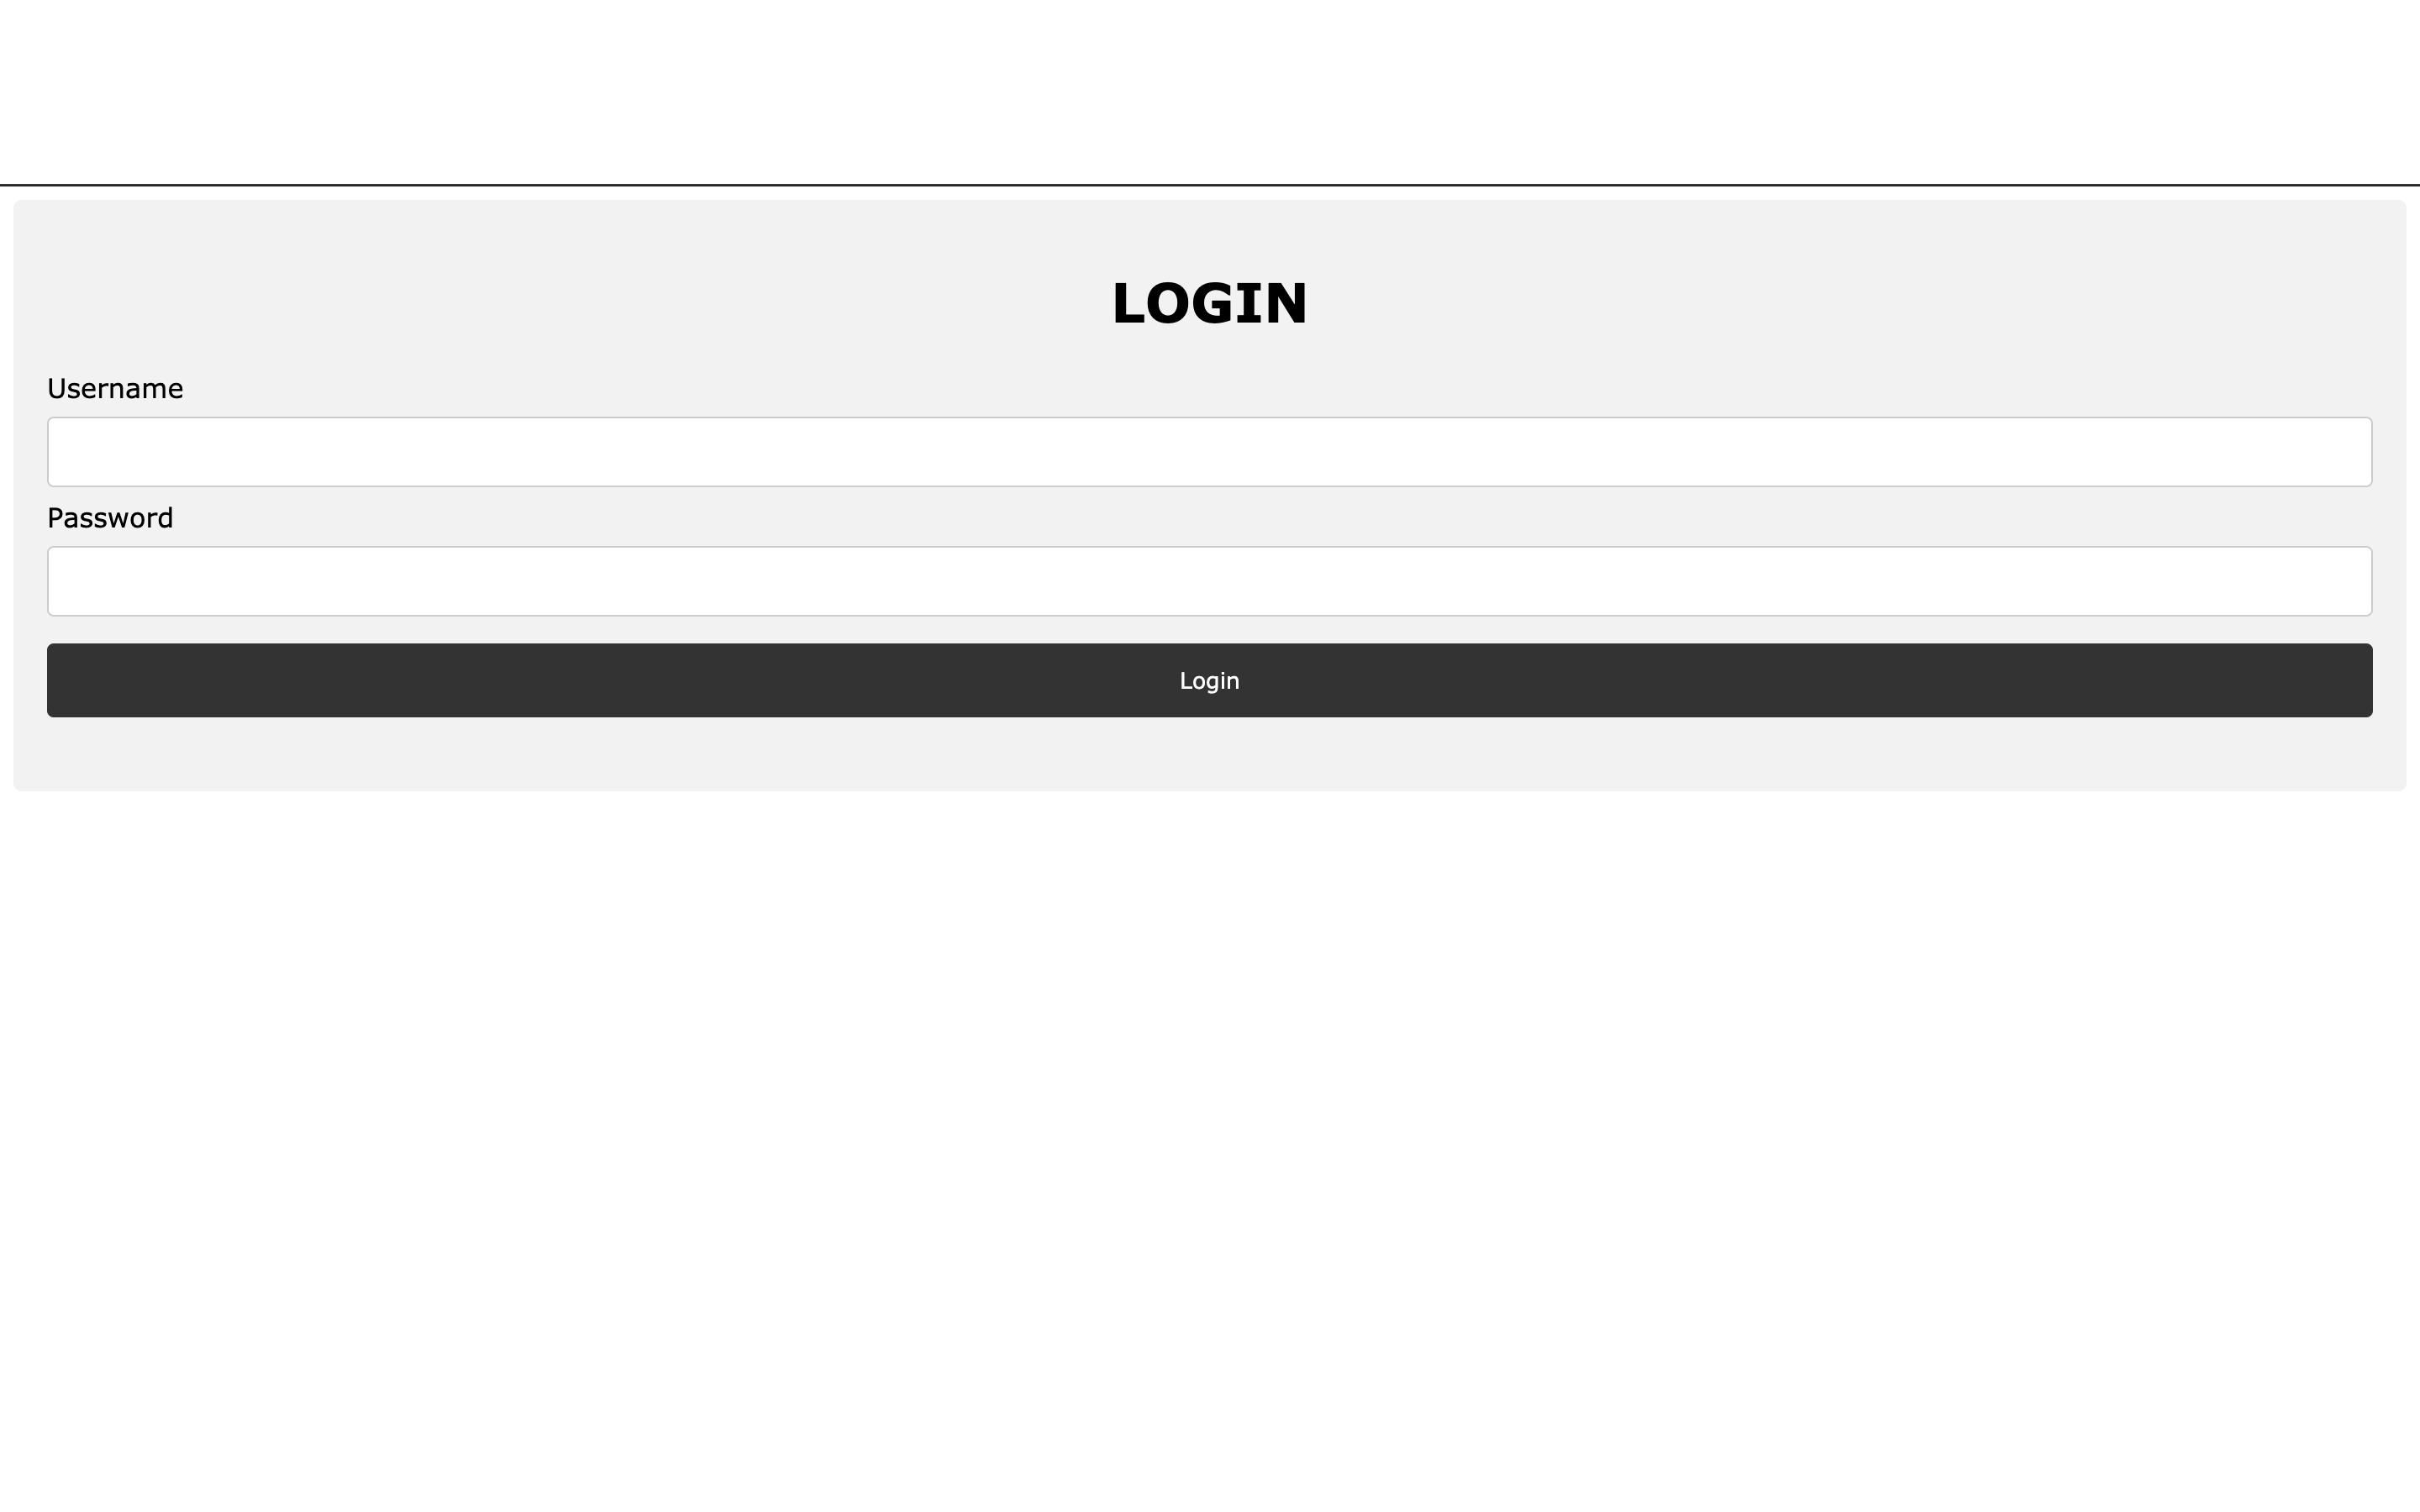
\includegraphics[scale=0.12]{res/images/login.png}
    \caption{Schermata di login}
\end{figure}
Nel caso le credenziali inserite non risultino corrette, sarà visualizzato un messaggio d'errore e sarà quindi necessario inserire di nuovo i dati.
\begin{figure}[H]
    \centering
    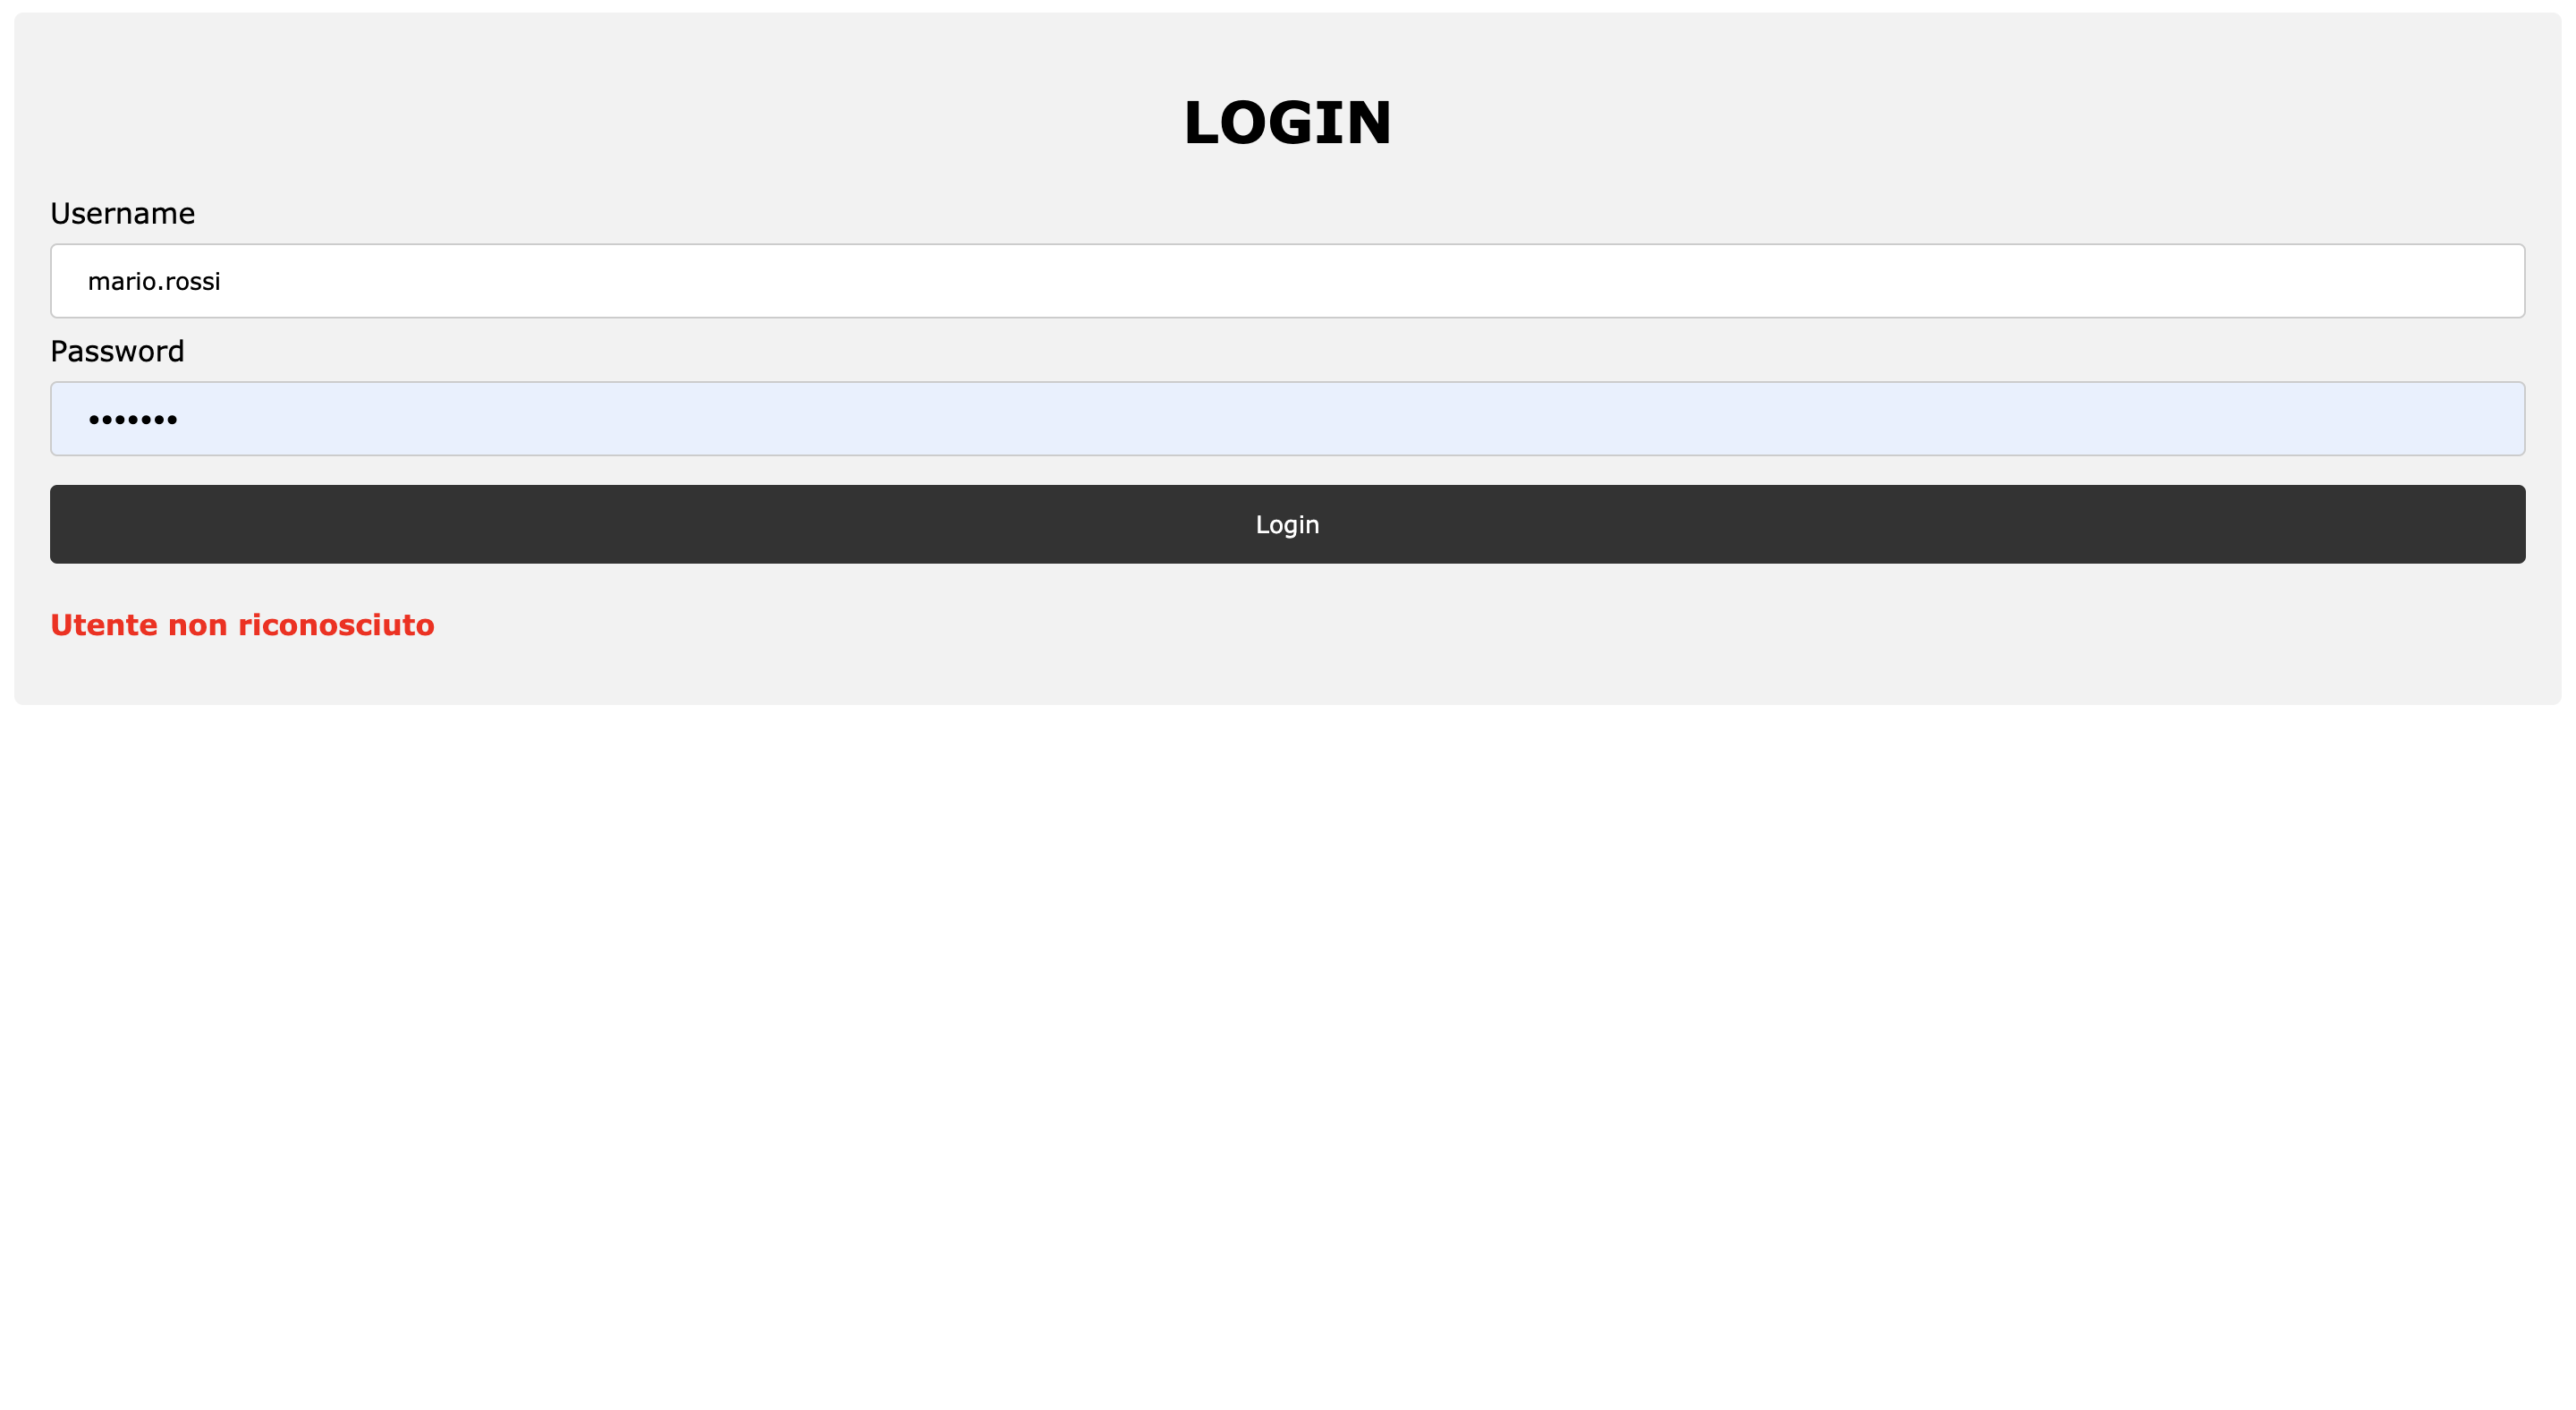
\includegraphics[scale=0.2]{res/images/login_errato.png}
    \caption{Schermata di login con errore}
\end{figure}

\subsection{Visualizzazione situazione in real time del magazzino}
\begin{itemize}
    \item Dopo l'autenticazione, tramite il menù selezionare il pulsante "Mappa";
    \begin{figure}[H]
        \centering
        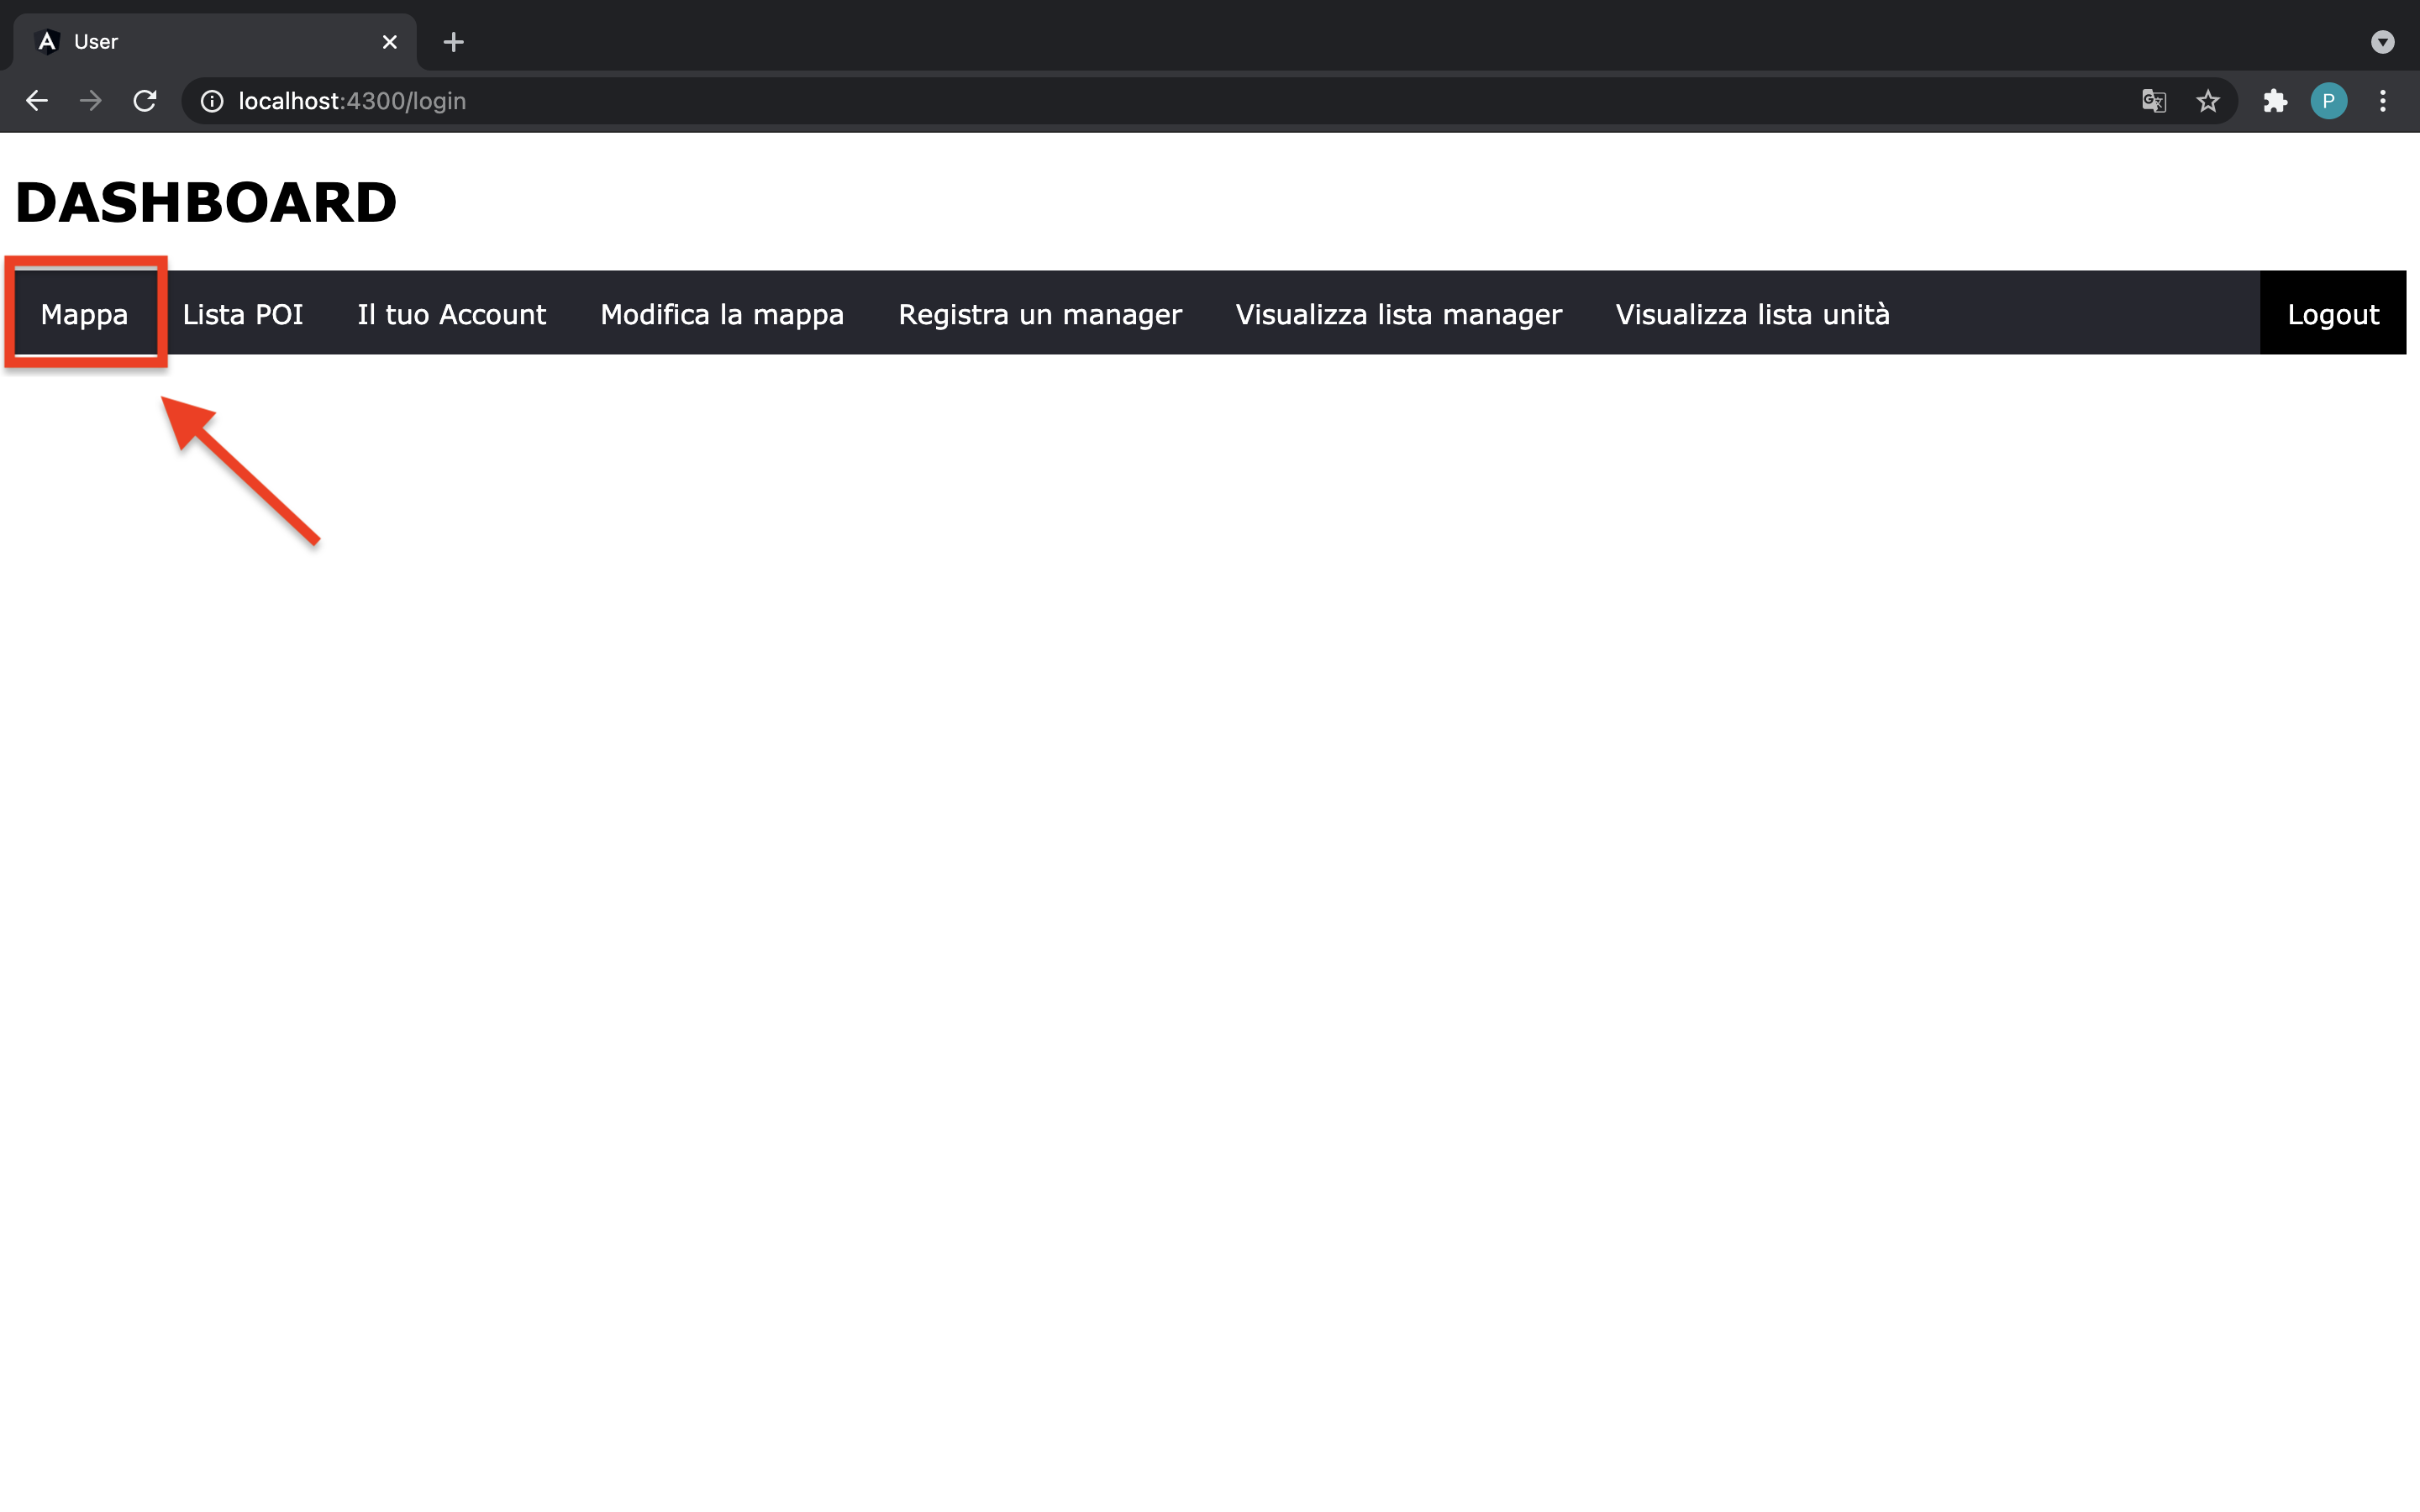
\includegraphics[scale=0.2]{res/images/dashboard1.png}
        \caption{Schermata dashboard con indicazione per visualizzare la mappa in real time}
    \end{figure}
    \item viene visualizzata la planimetria del magazzino e la rappresentazione dei muletti che si spostano tramite l'icona blu e il proprio id;
    \item la tabella a destra rappresenta le liste di task con i relativi muletti che le stanno soddisfando.
    
\end{itemize}

\begin{figure}[H]
    \centering
    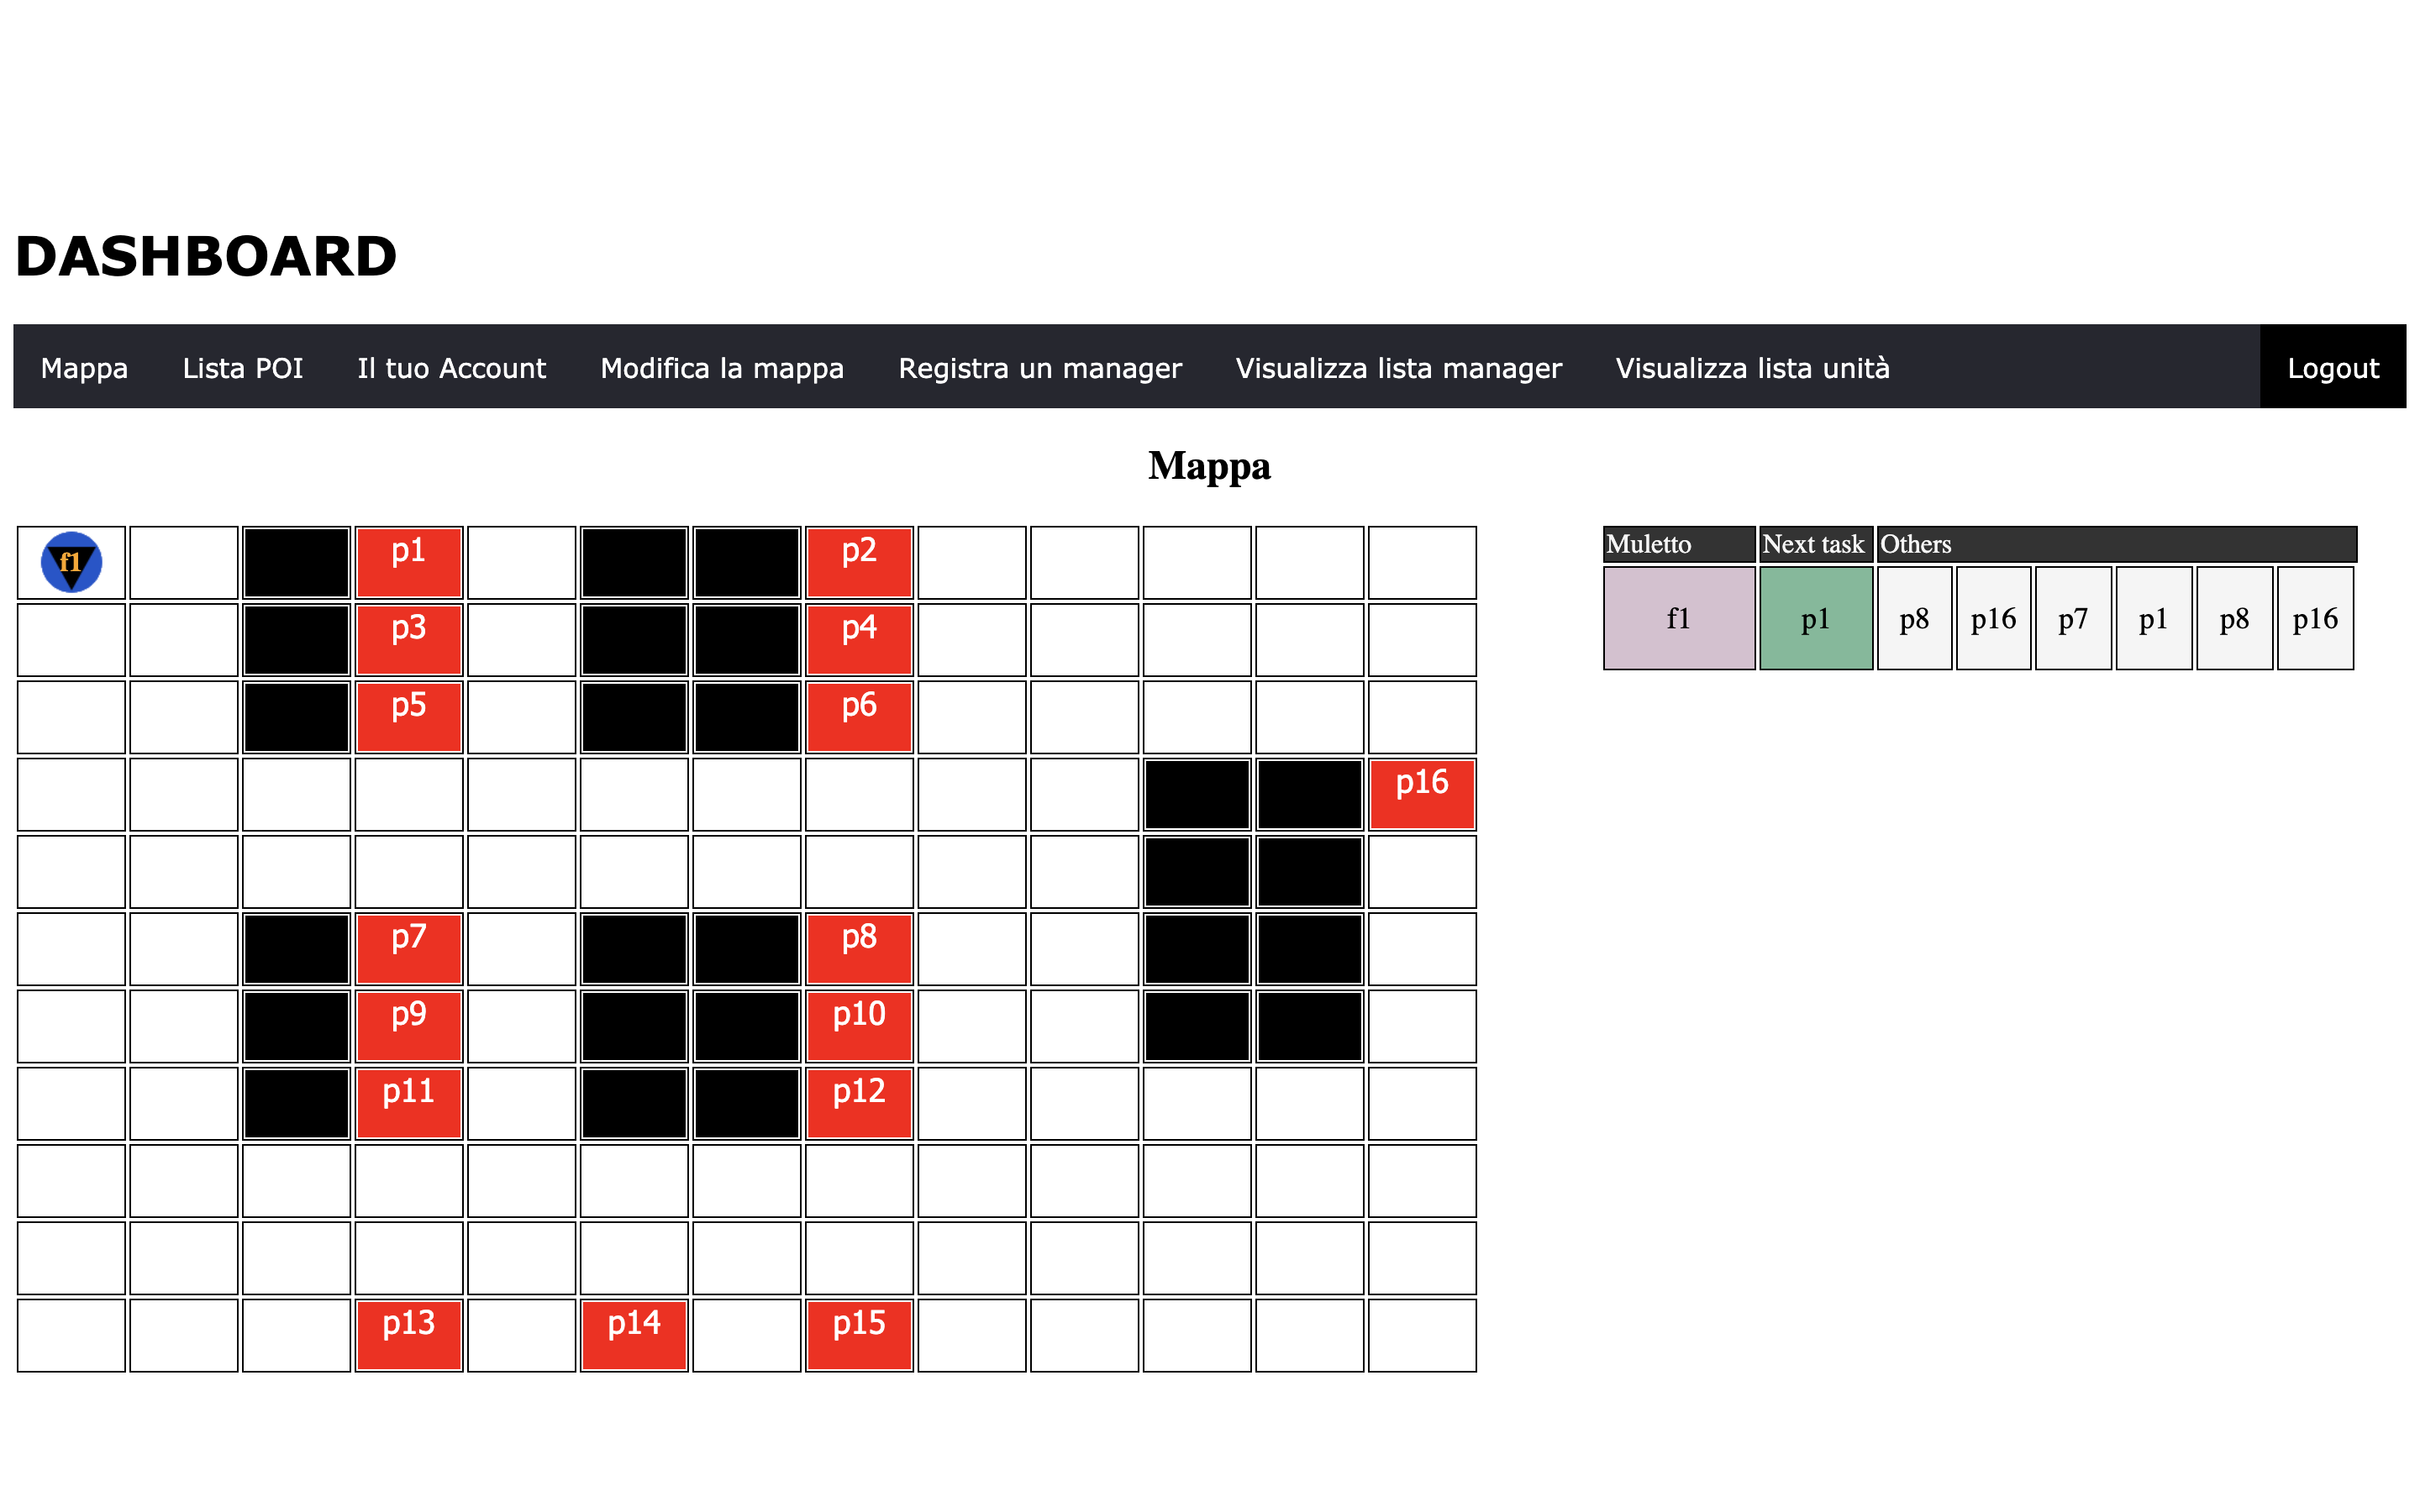
\includegraphics[scale=0.2]{res/images/map_user.png}
    \caption{Schermata visualizzazione in real time del magazzino}
\end{figure}

\subsection{Visualizzazione lista completa punti di interesse}
\begin{itemize}
    \item Dopo l'autenticazione, tramite il menù selezionare il pulsante "Lista POI";
    \begin{figure}[H]
        \centering
        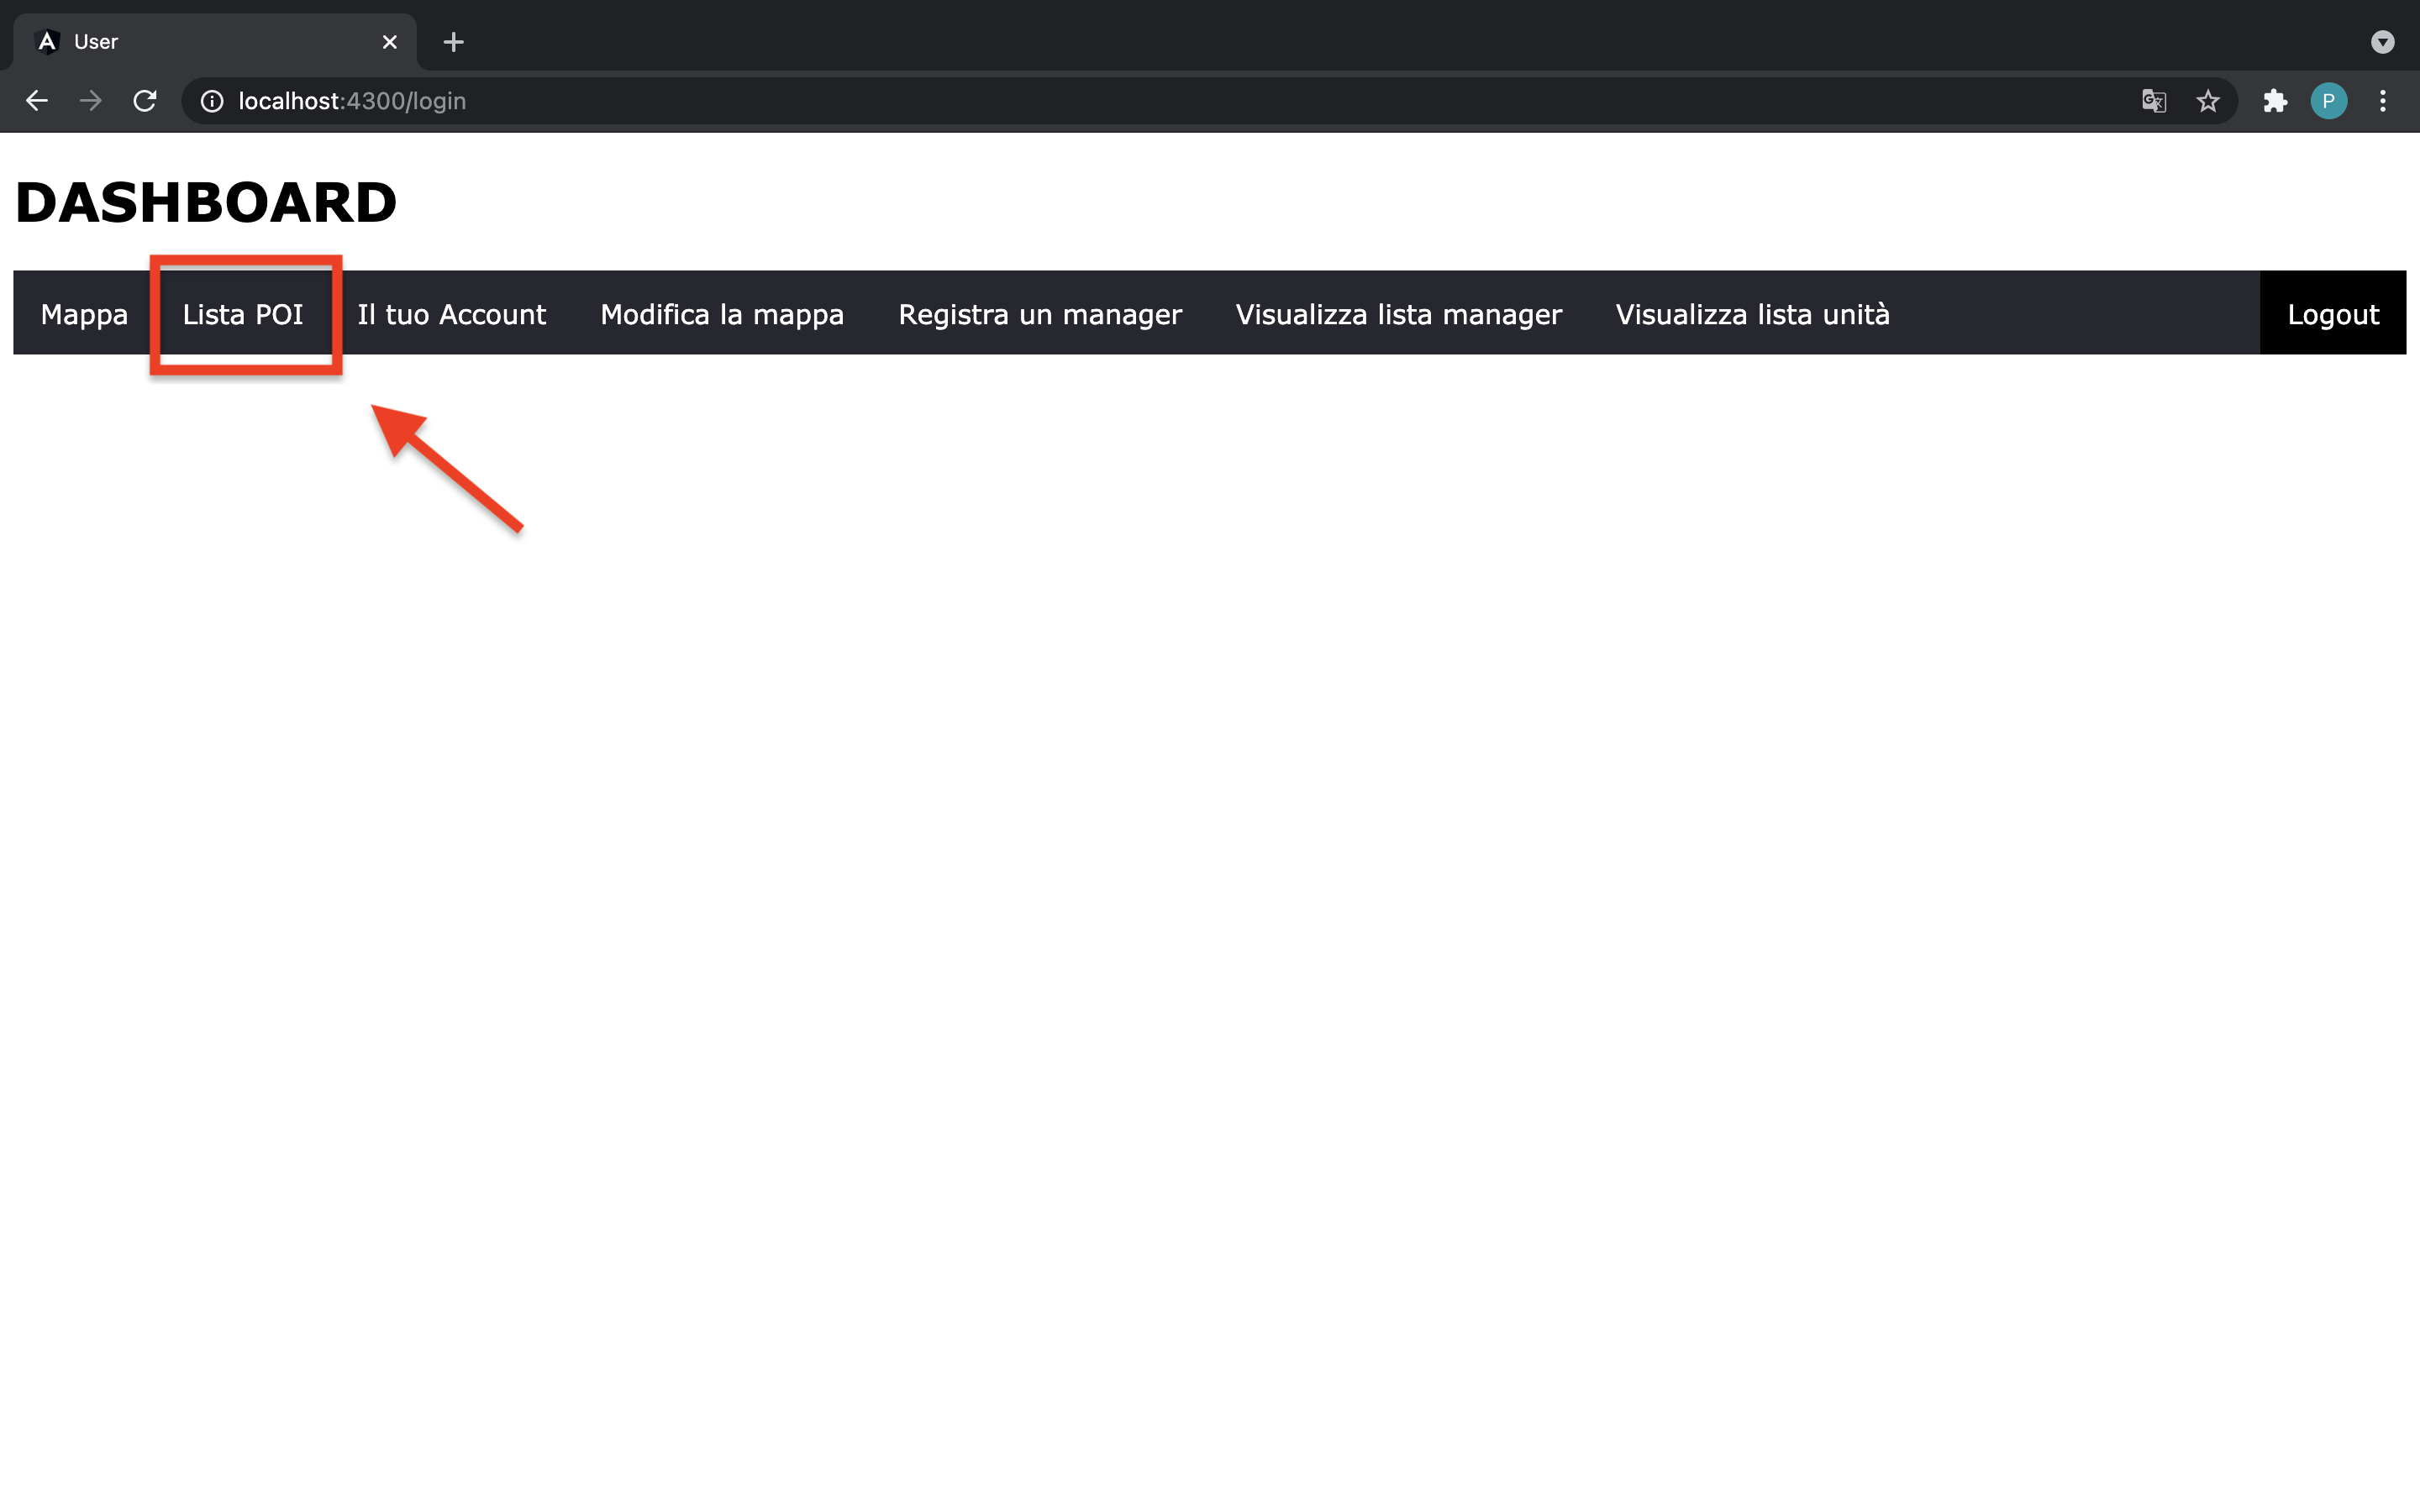
\includegraphics[scale=0.2]{res/images/dashboard2.png}
        \caption{Schermata dashboard con indicazione per la visualizzazione di tutti i POI}
    \end{figure}
    \item si viene indirizzati alla pagina con l'elenco di tutti i punti di interesse presenti nel magazzino con il relativo id e nome.

\end{itemize}

\begin{figure}[H]
    \centering
    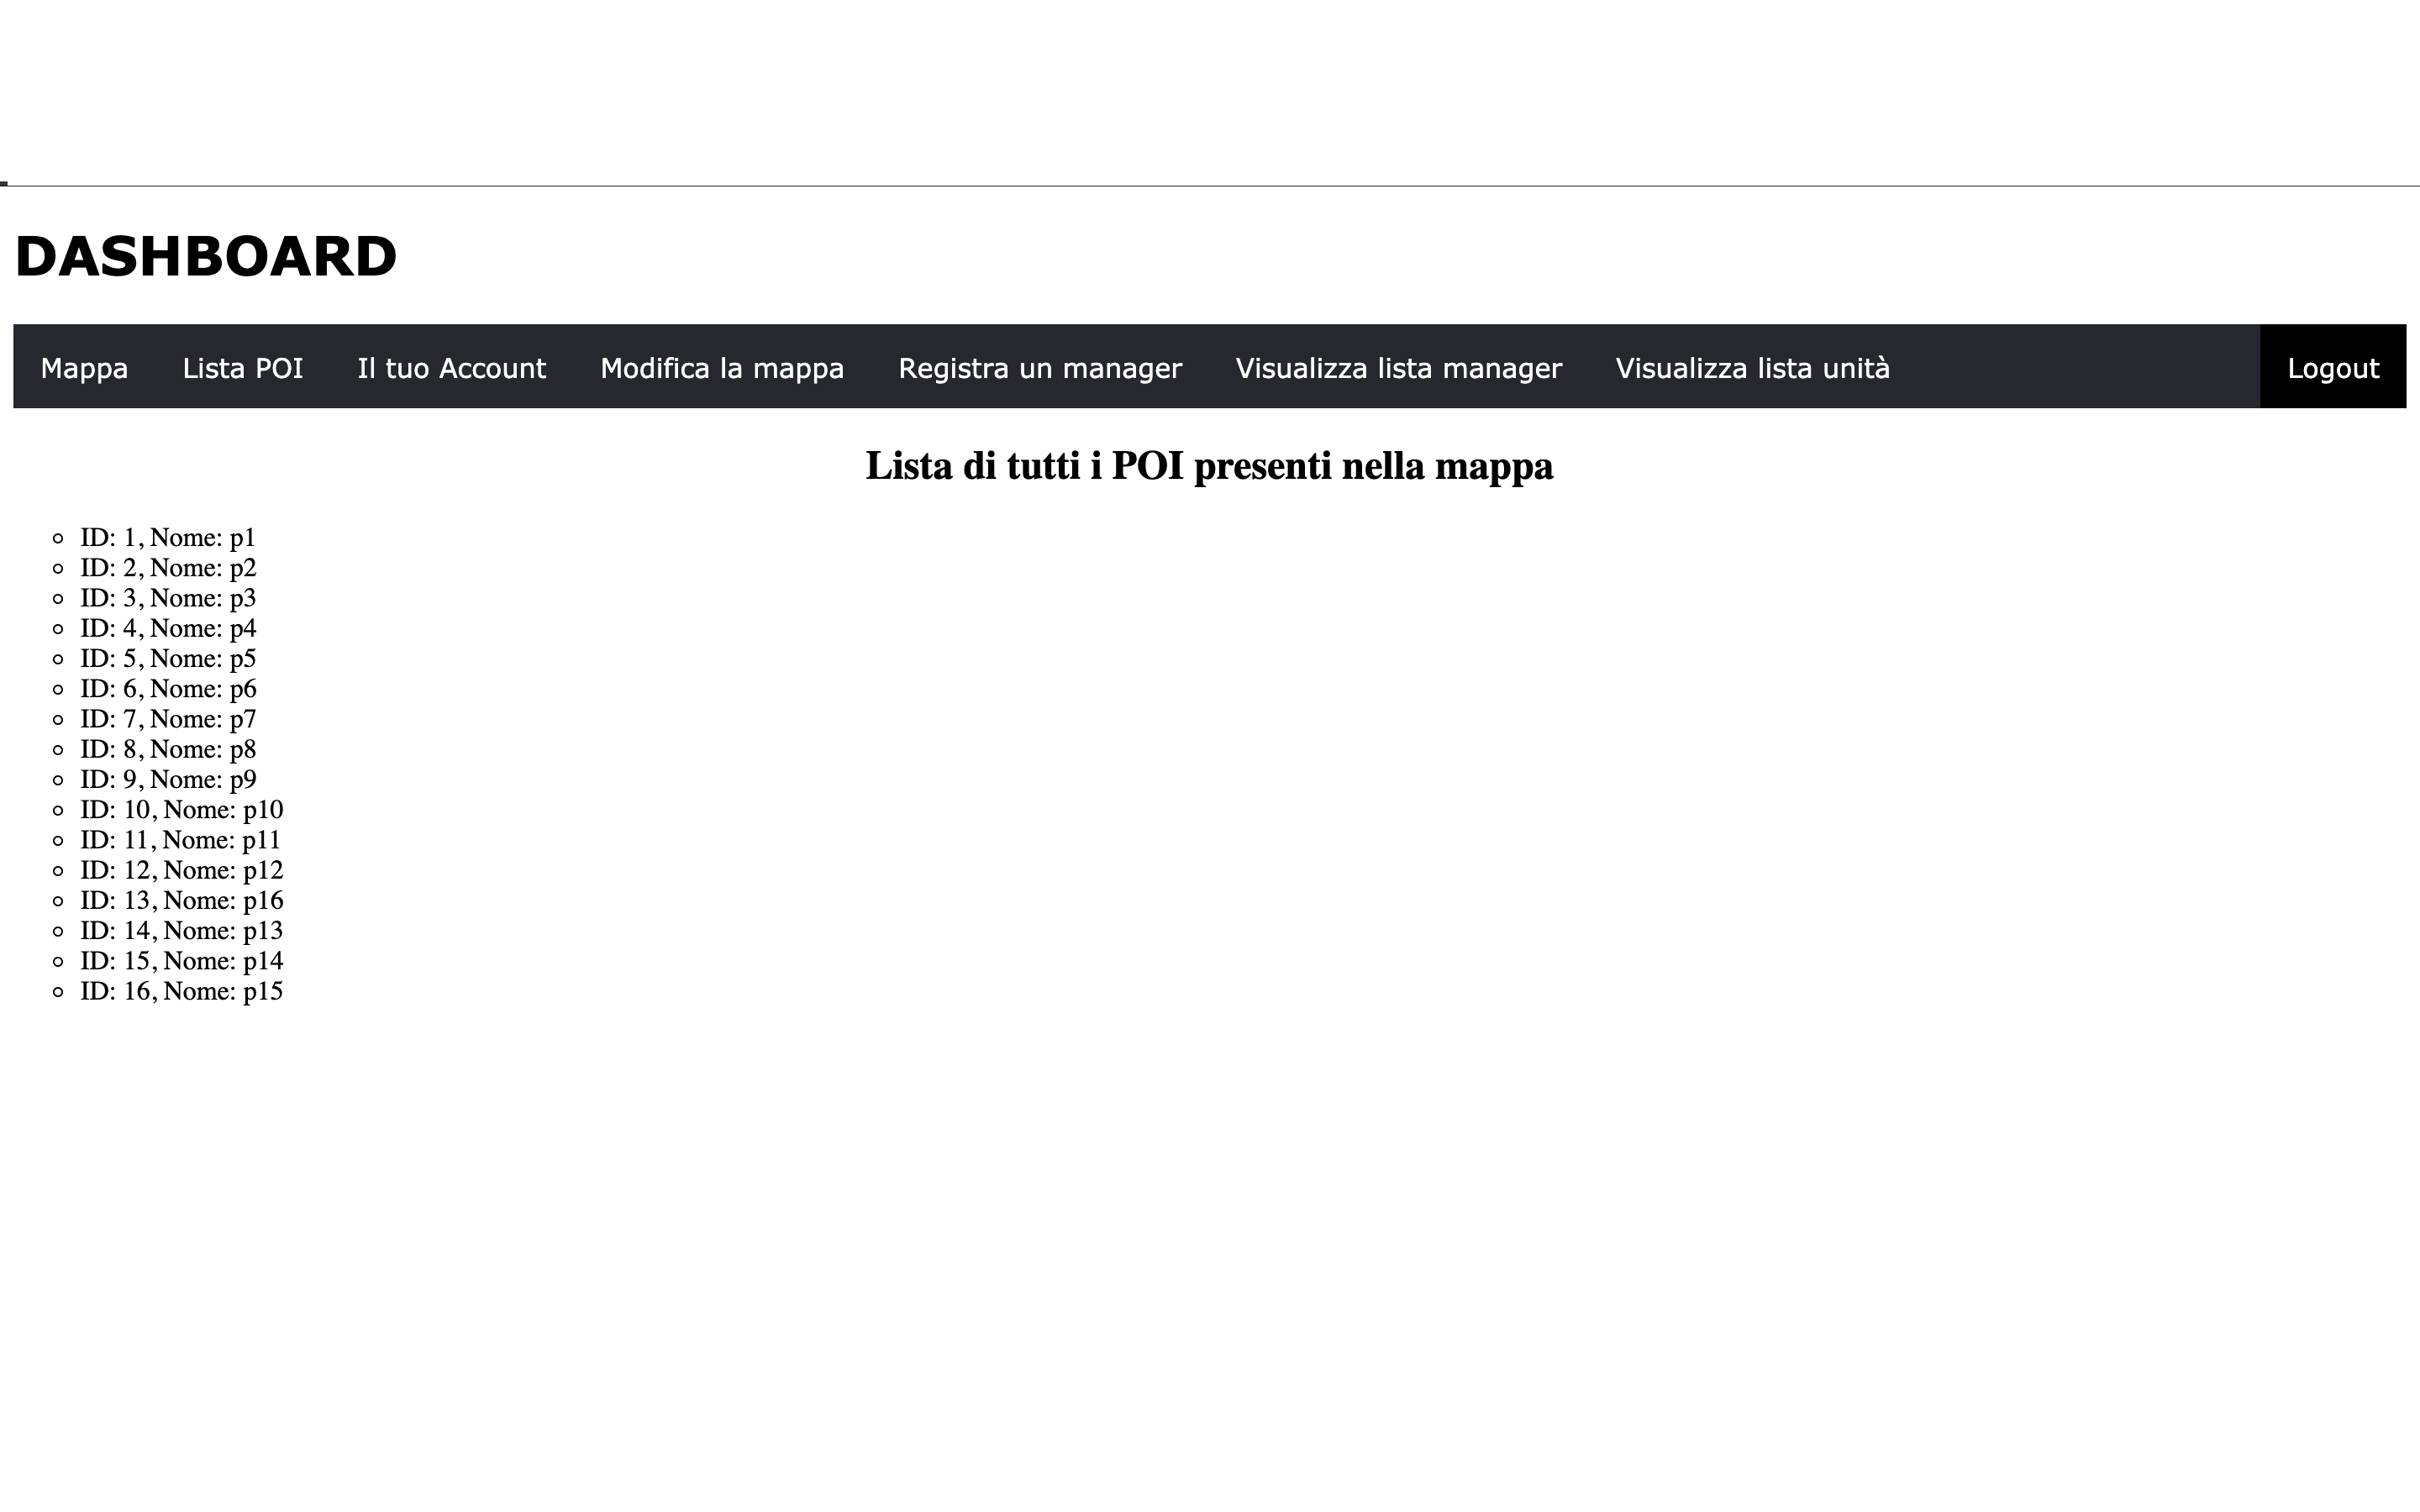
\includegraphics[scale=0.2]{res/images/listpoi_user.png}
    \caption{Schermata visualizzazione lista punti di interesse}
\end{figure}

\subsection{Visualizzazione dati del proprio profilo e modifica}
\begin{itemize}
    \item Dopo l'autenticazione, tramite il menù selezionare il pulsante "Il tuo account";
    \begin{figure}[H]
        \centering
        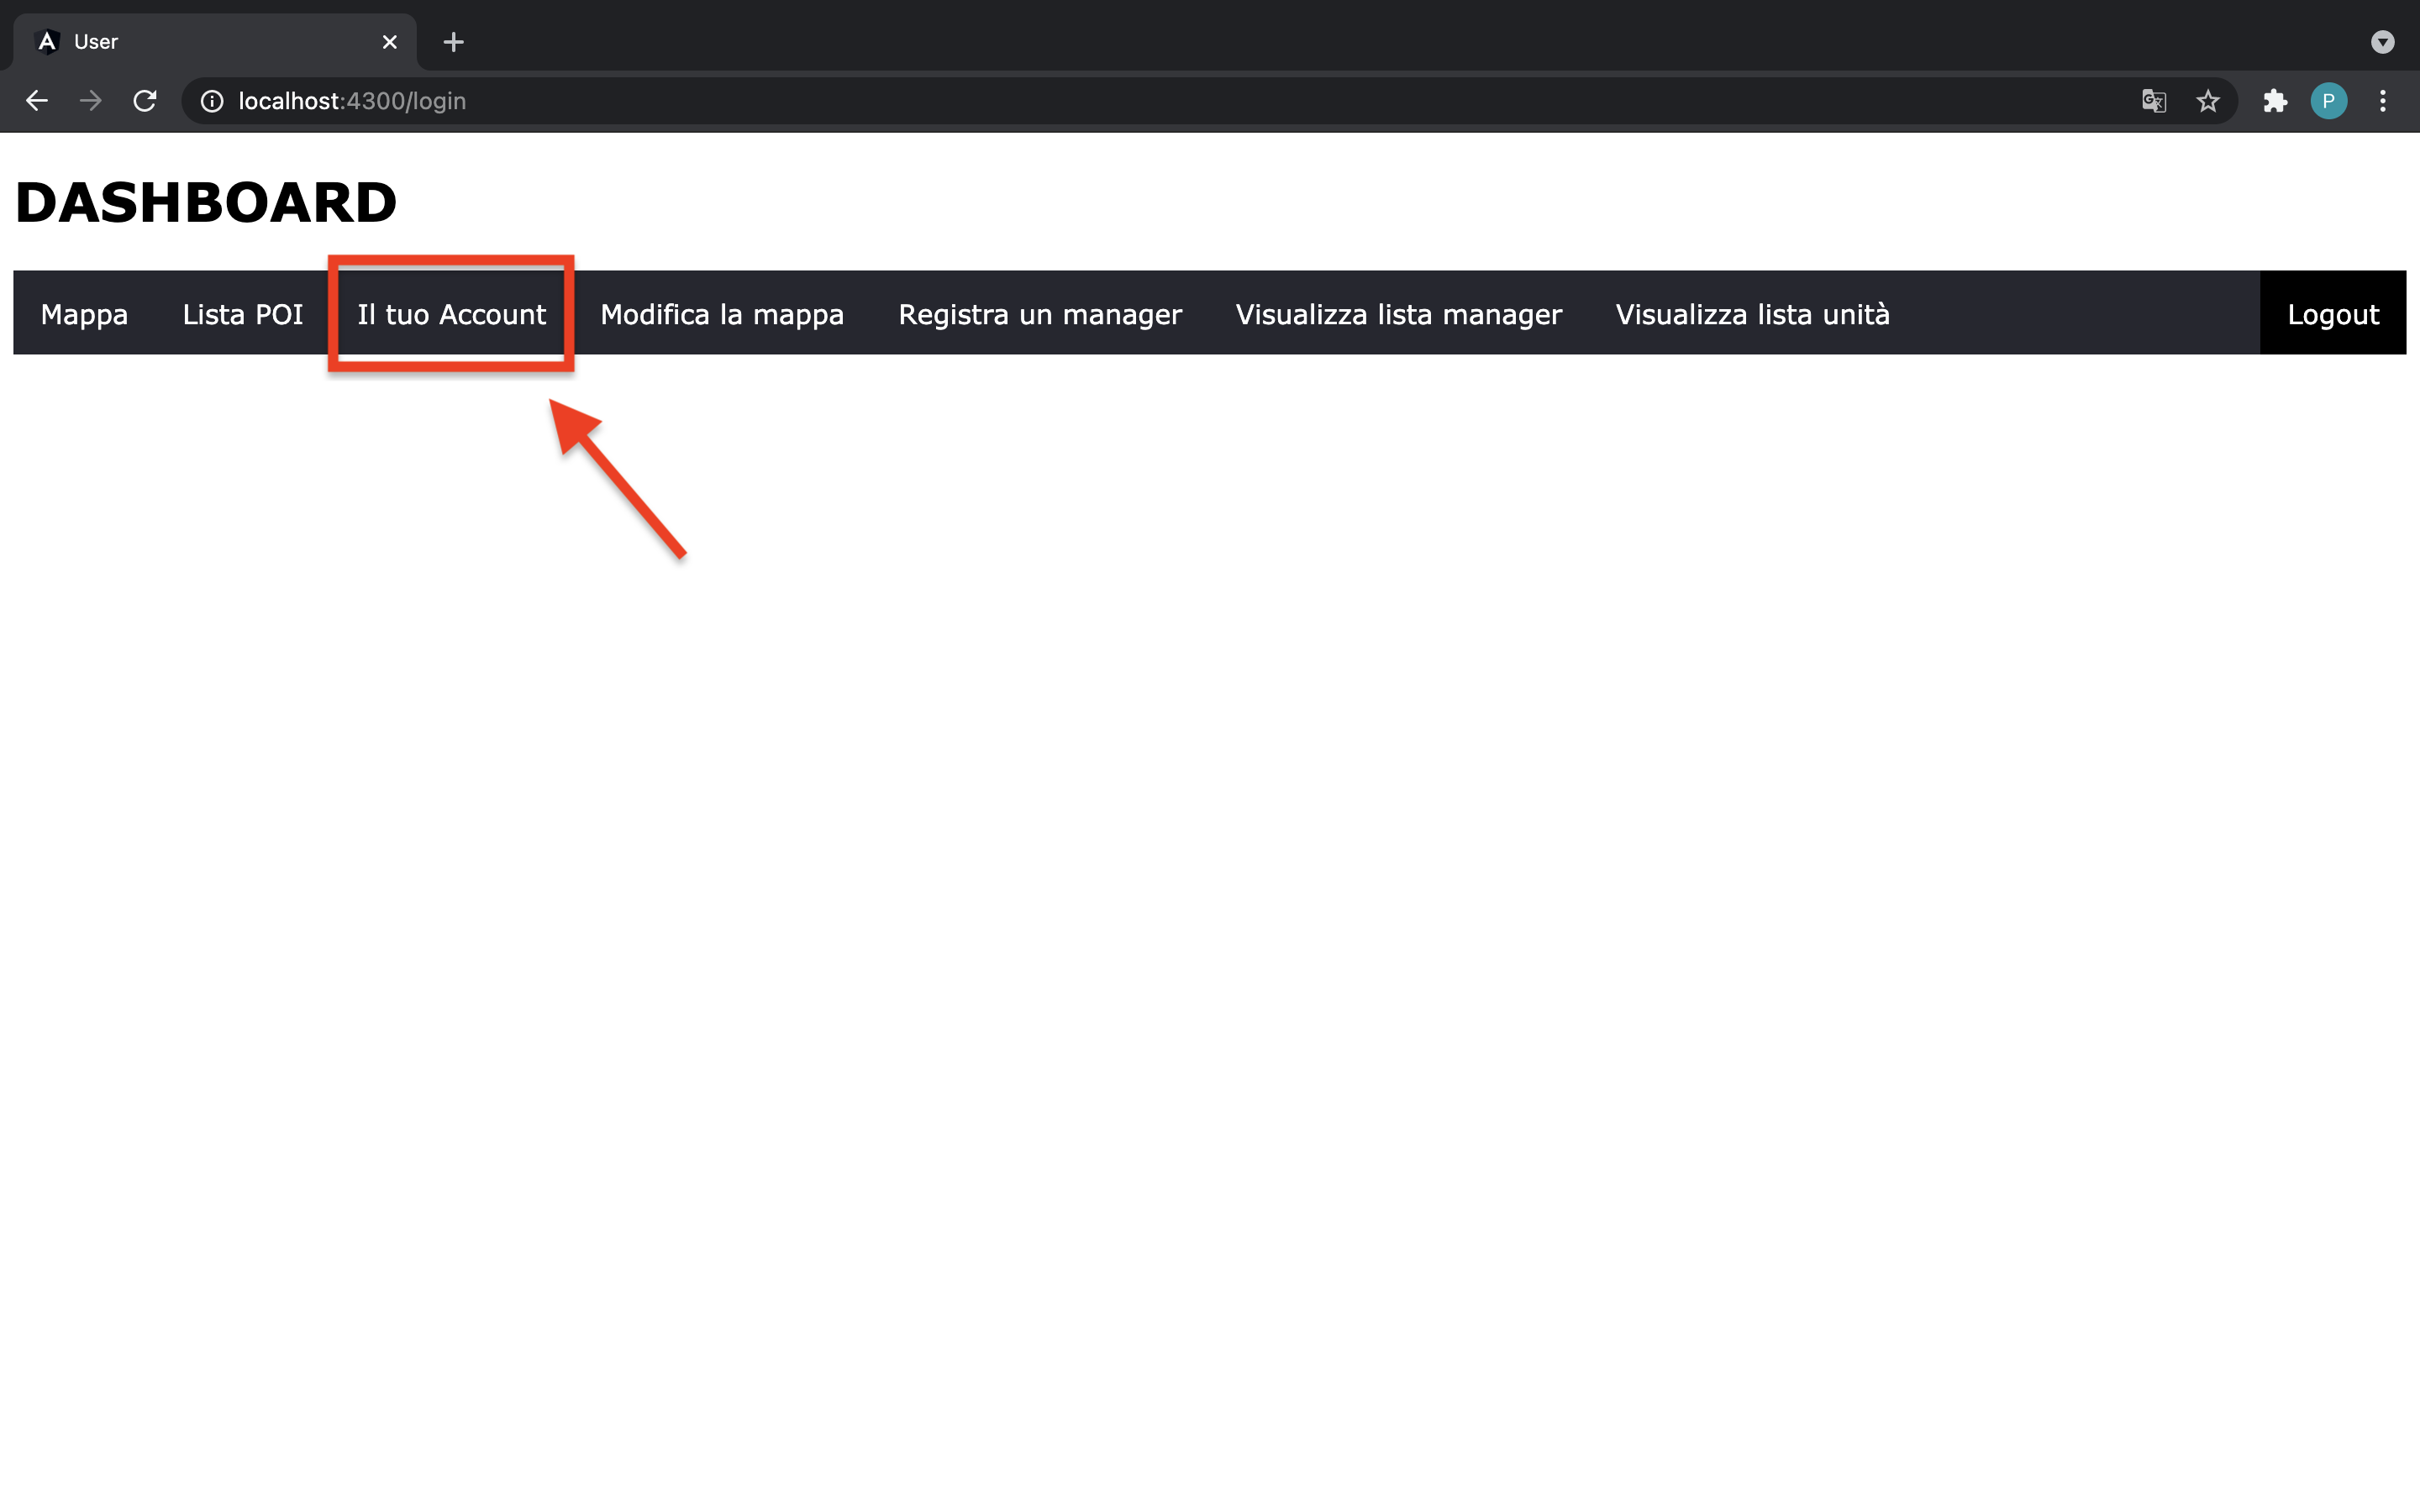
\includegraphics[scale=0.2]{res/images/dashboard3.png}
        \caption{Schermata dashboard con indicazione per la visualizzazione del proprio profilo}
    \end{figure}
    
    \item si viene indirizzati alla pagina con i propri dati utente: Name, Surname, Password;
    \item se si desidera modificare alcuni campi, è necessario scrivere nell'apposito form i nuovi dati e premere il pulsante "Salva Modifiche".
    \begin{figure}[H]
        \centering
        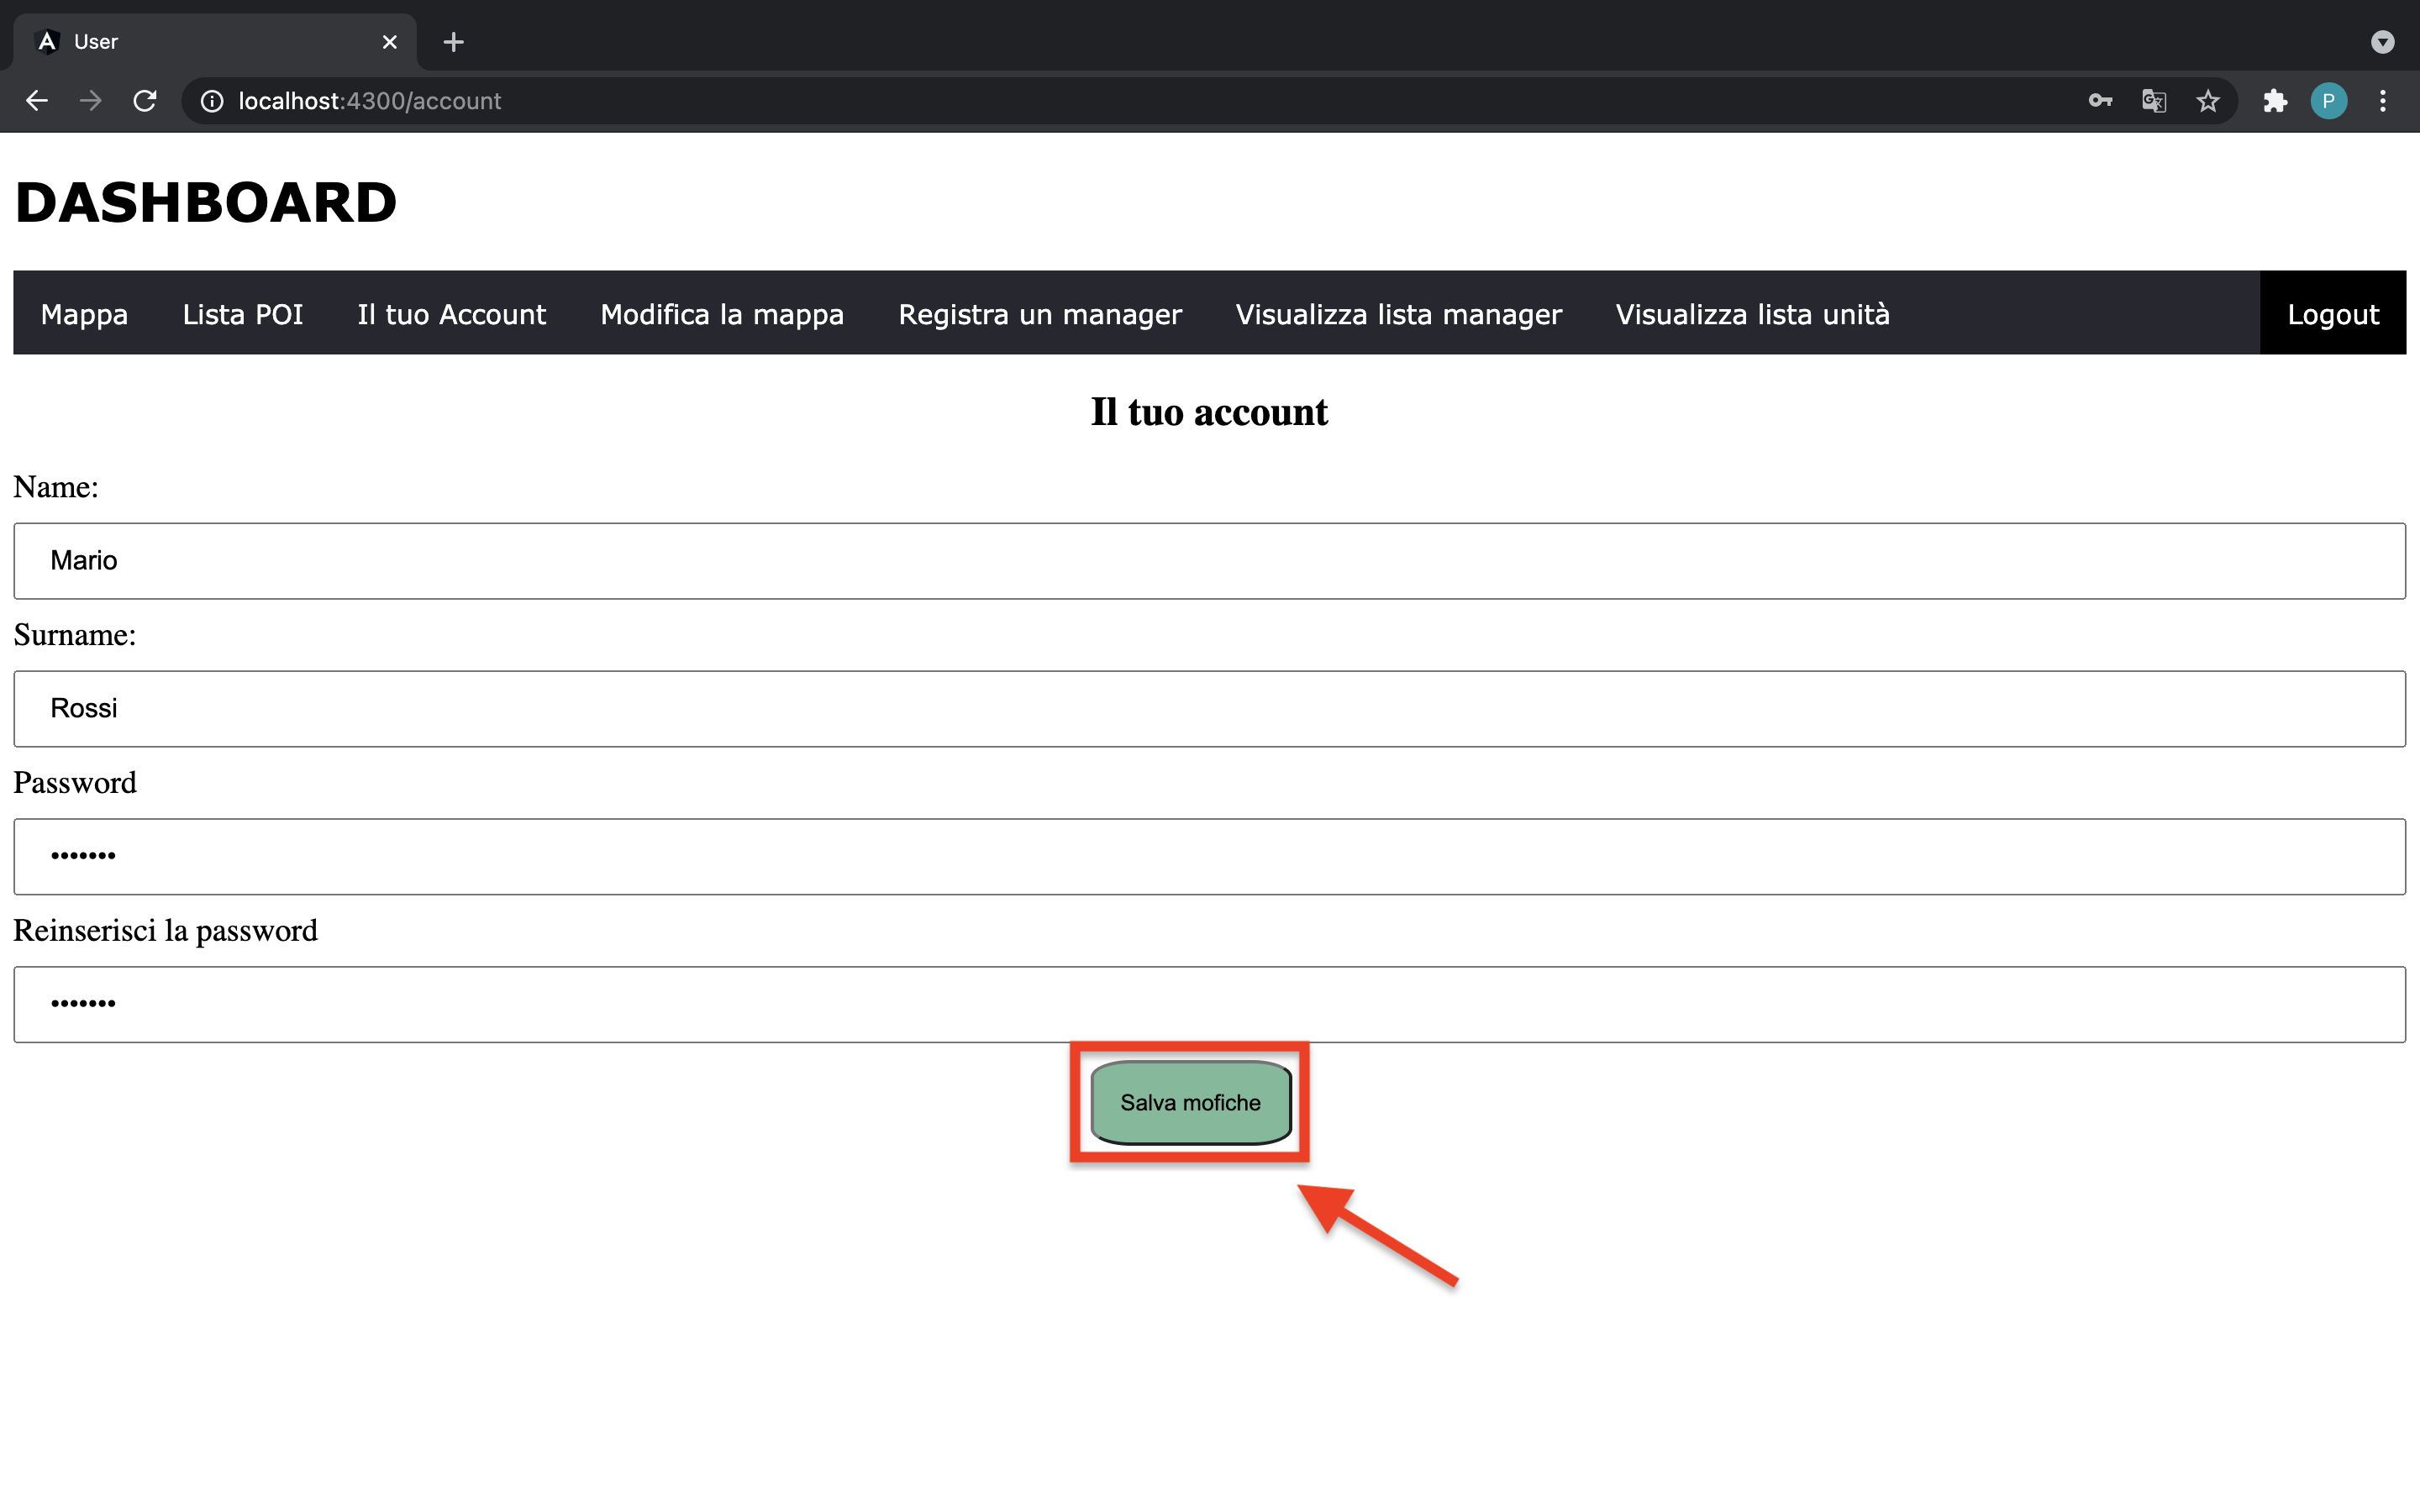
\includegraphics[scale=0.2]{res/images/account_user.png}
        \caption{Schermata proprio profilo}
    \end{figure}
    \item Se si intende cambiare la Password, l'inserimento nei due campi deve coincidere altrimenti si visualizzerà un errore.
    \begin{figure}[H]
        \centering
        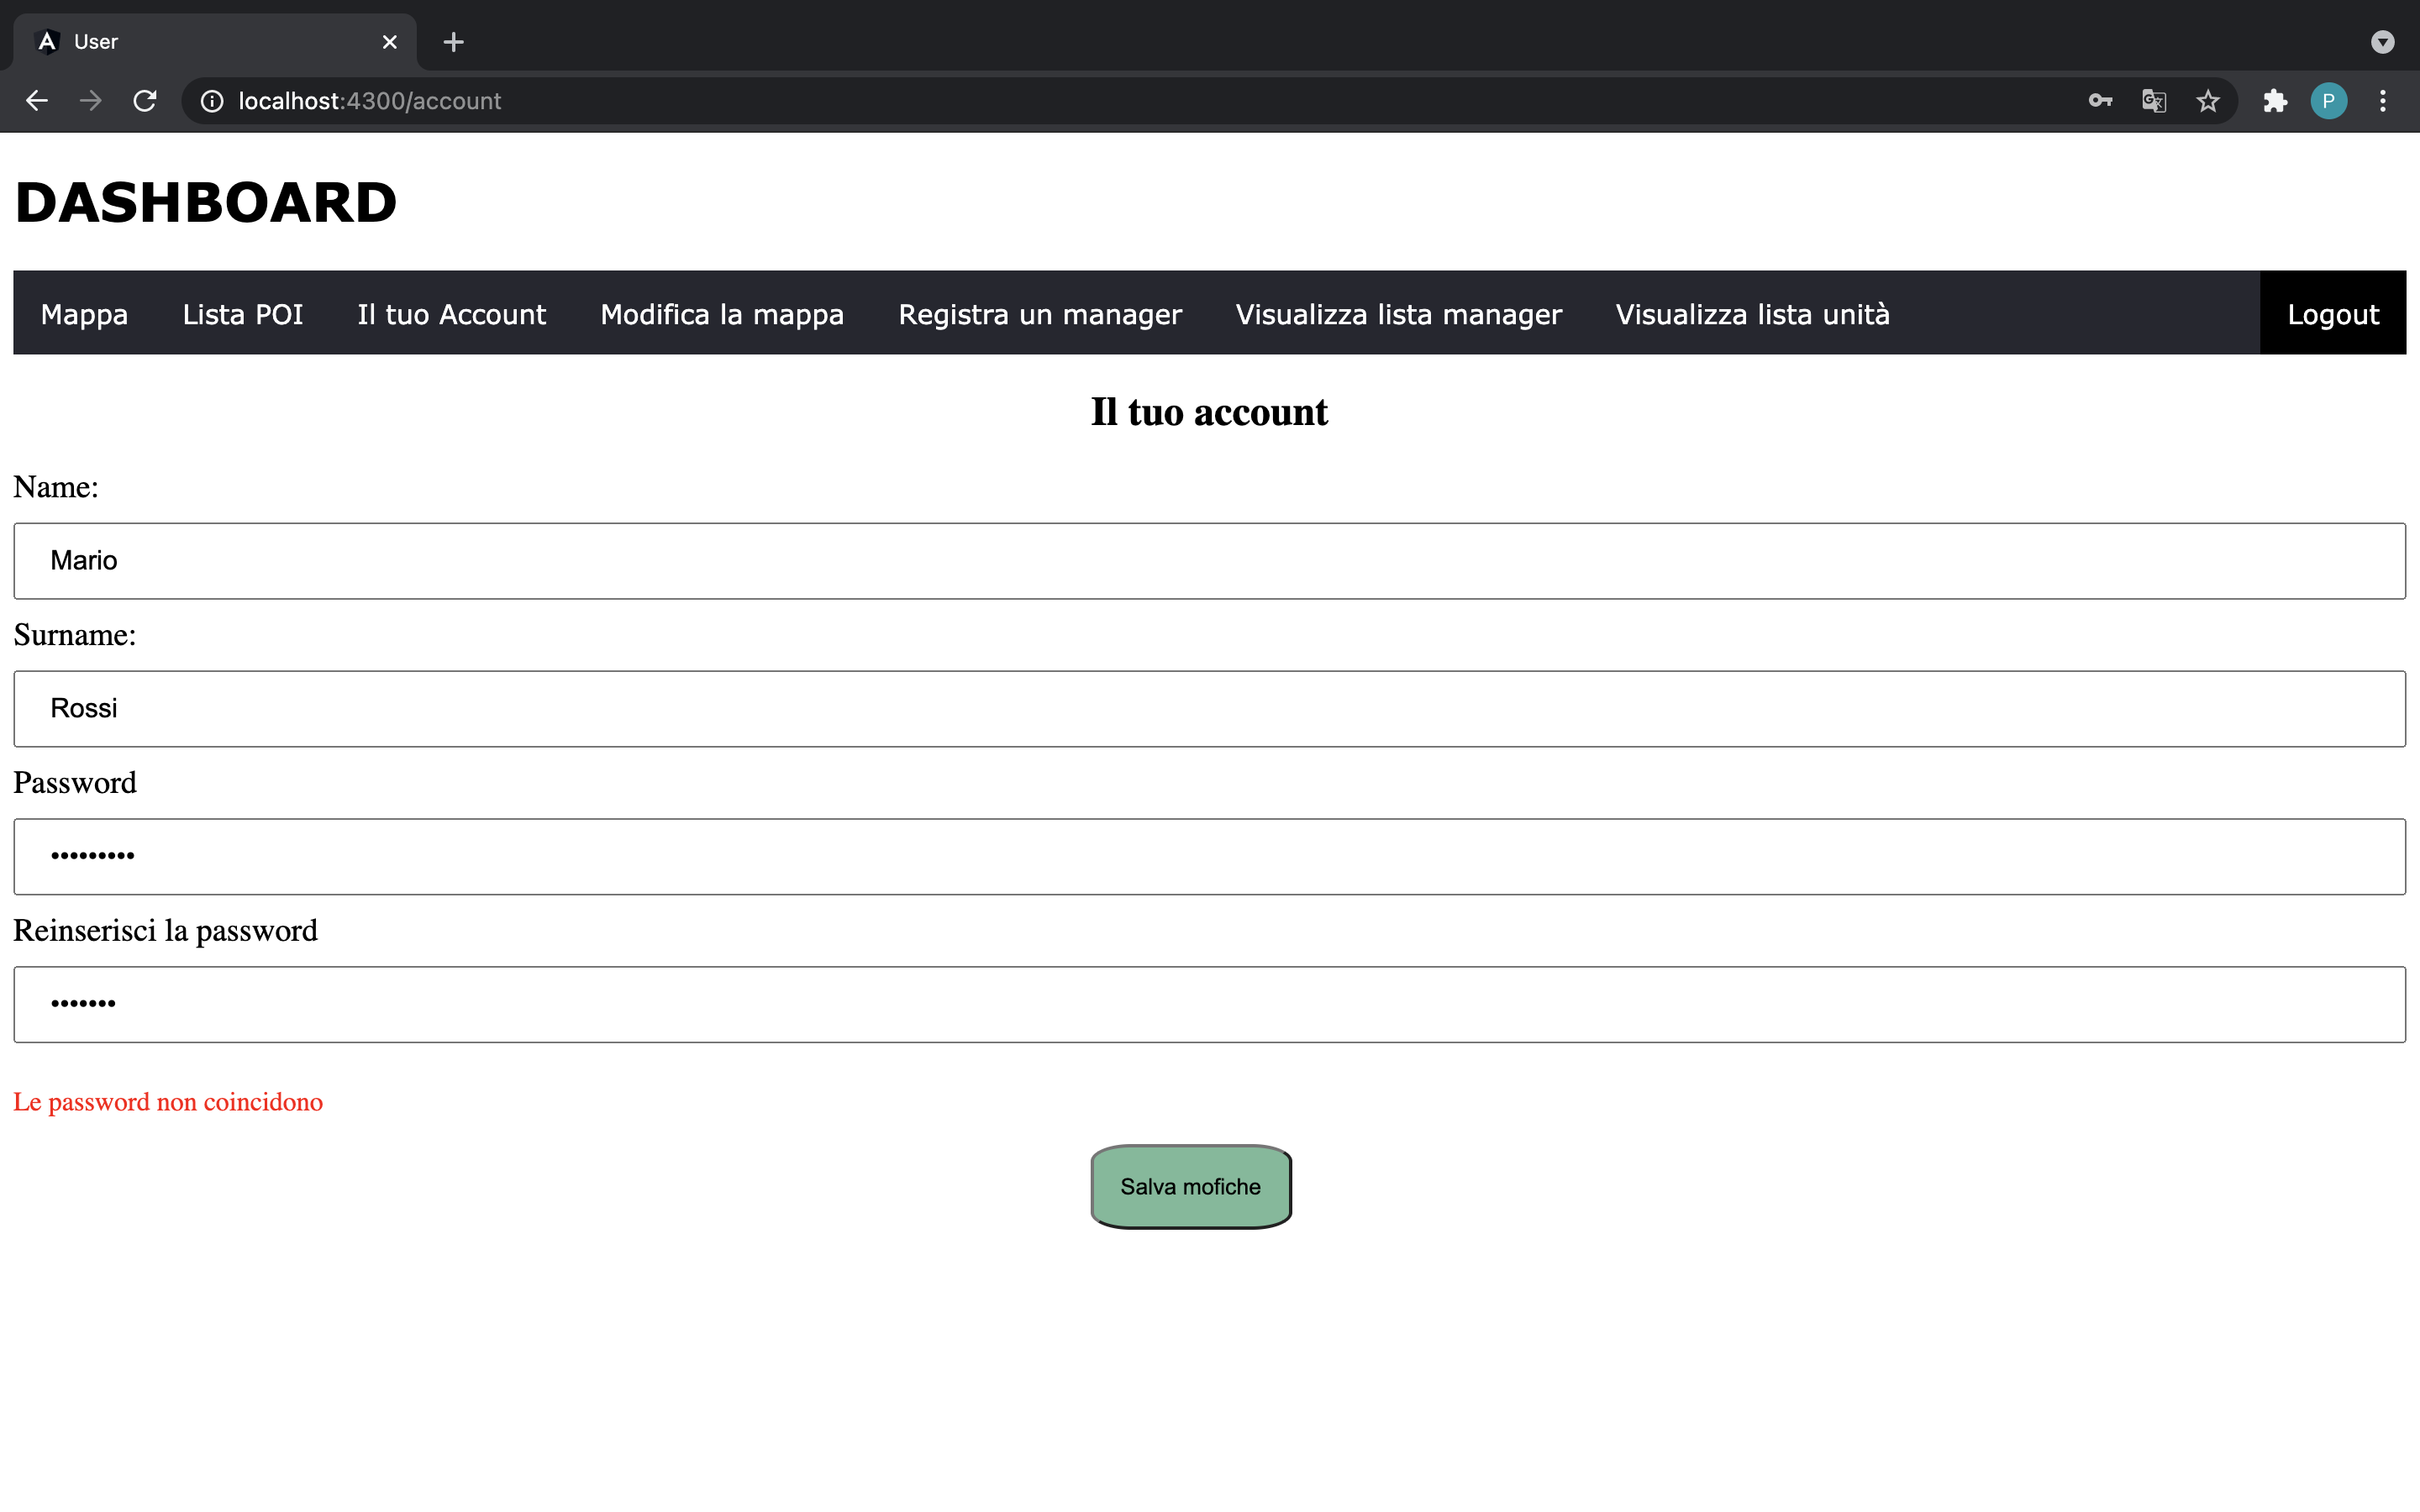
\includegraphics[scale=0.2]{res/images/account_errore.png}
        \caption{Schermata modifica
        password con messaggio d'errore}
    \end{figure}
\end{itemize}



\subsection{Visualizzazione liste di task}
\begin{itemize}
    \item Dopo l'autenticazione, tramite il menù selezionare il pulsante "Visualizza liste di task";
    \begin{figure}[H]
        \centering
        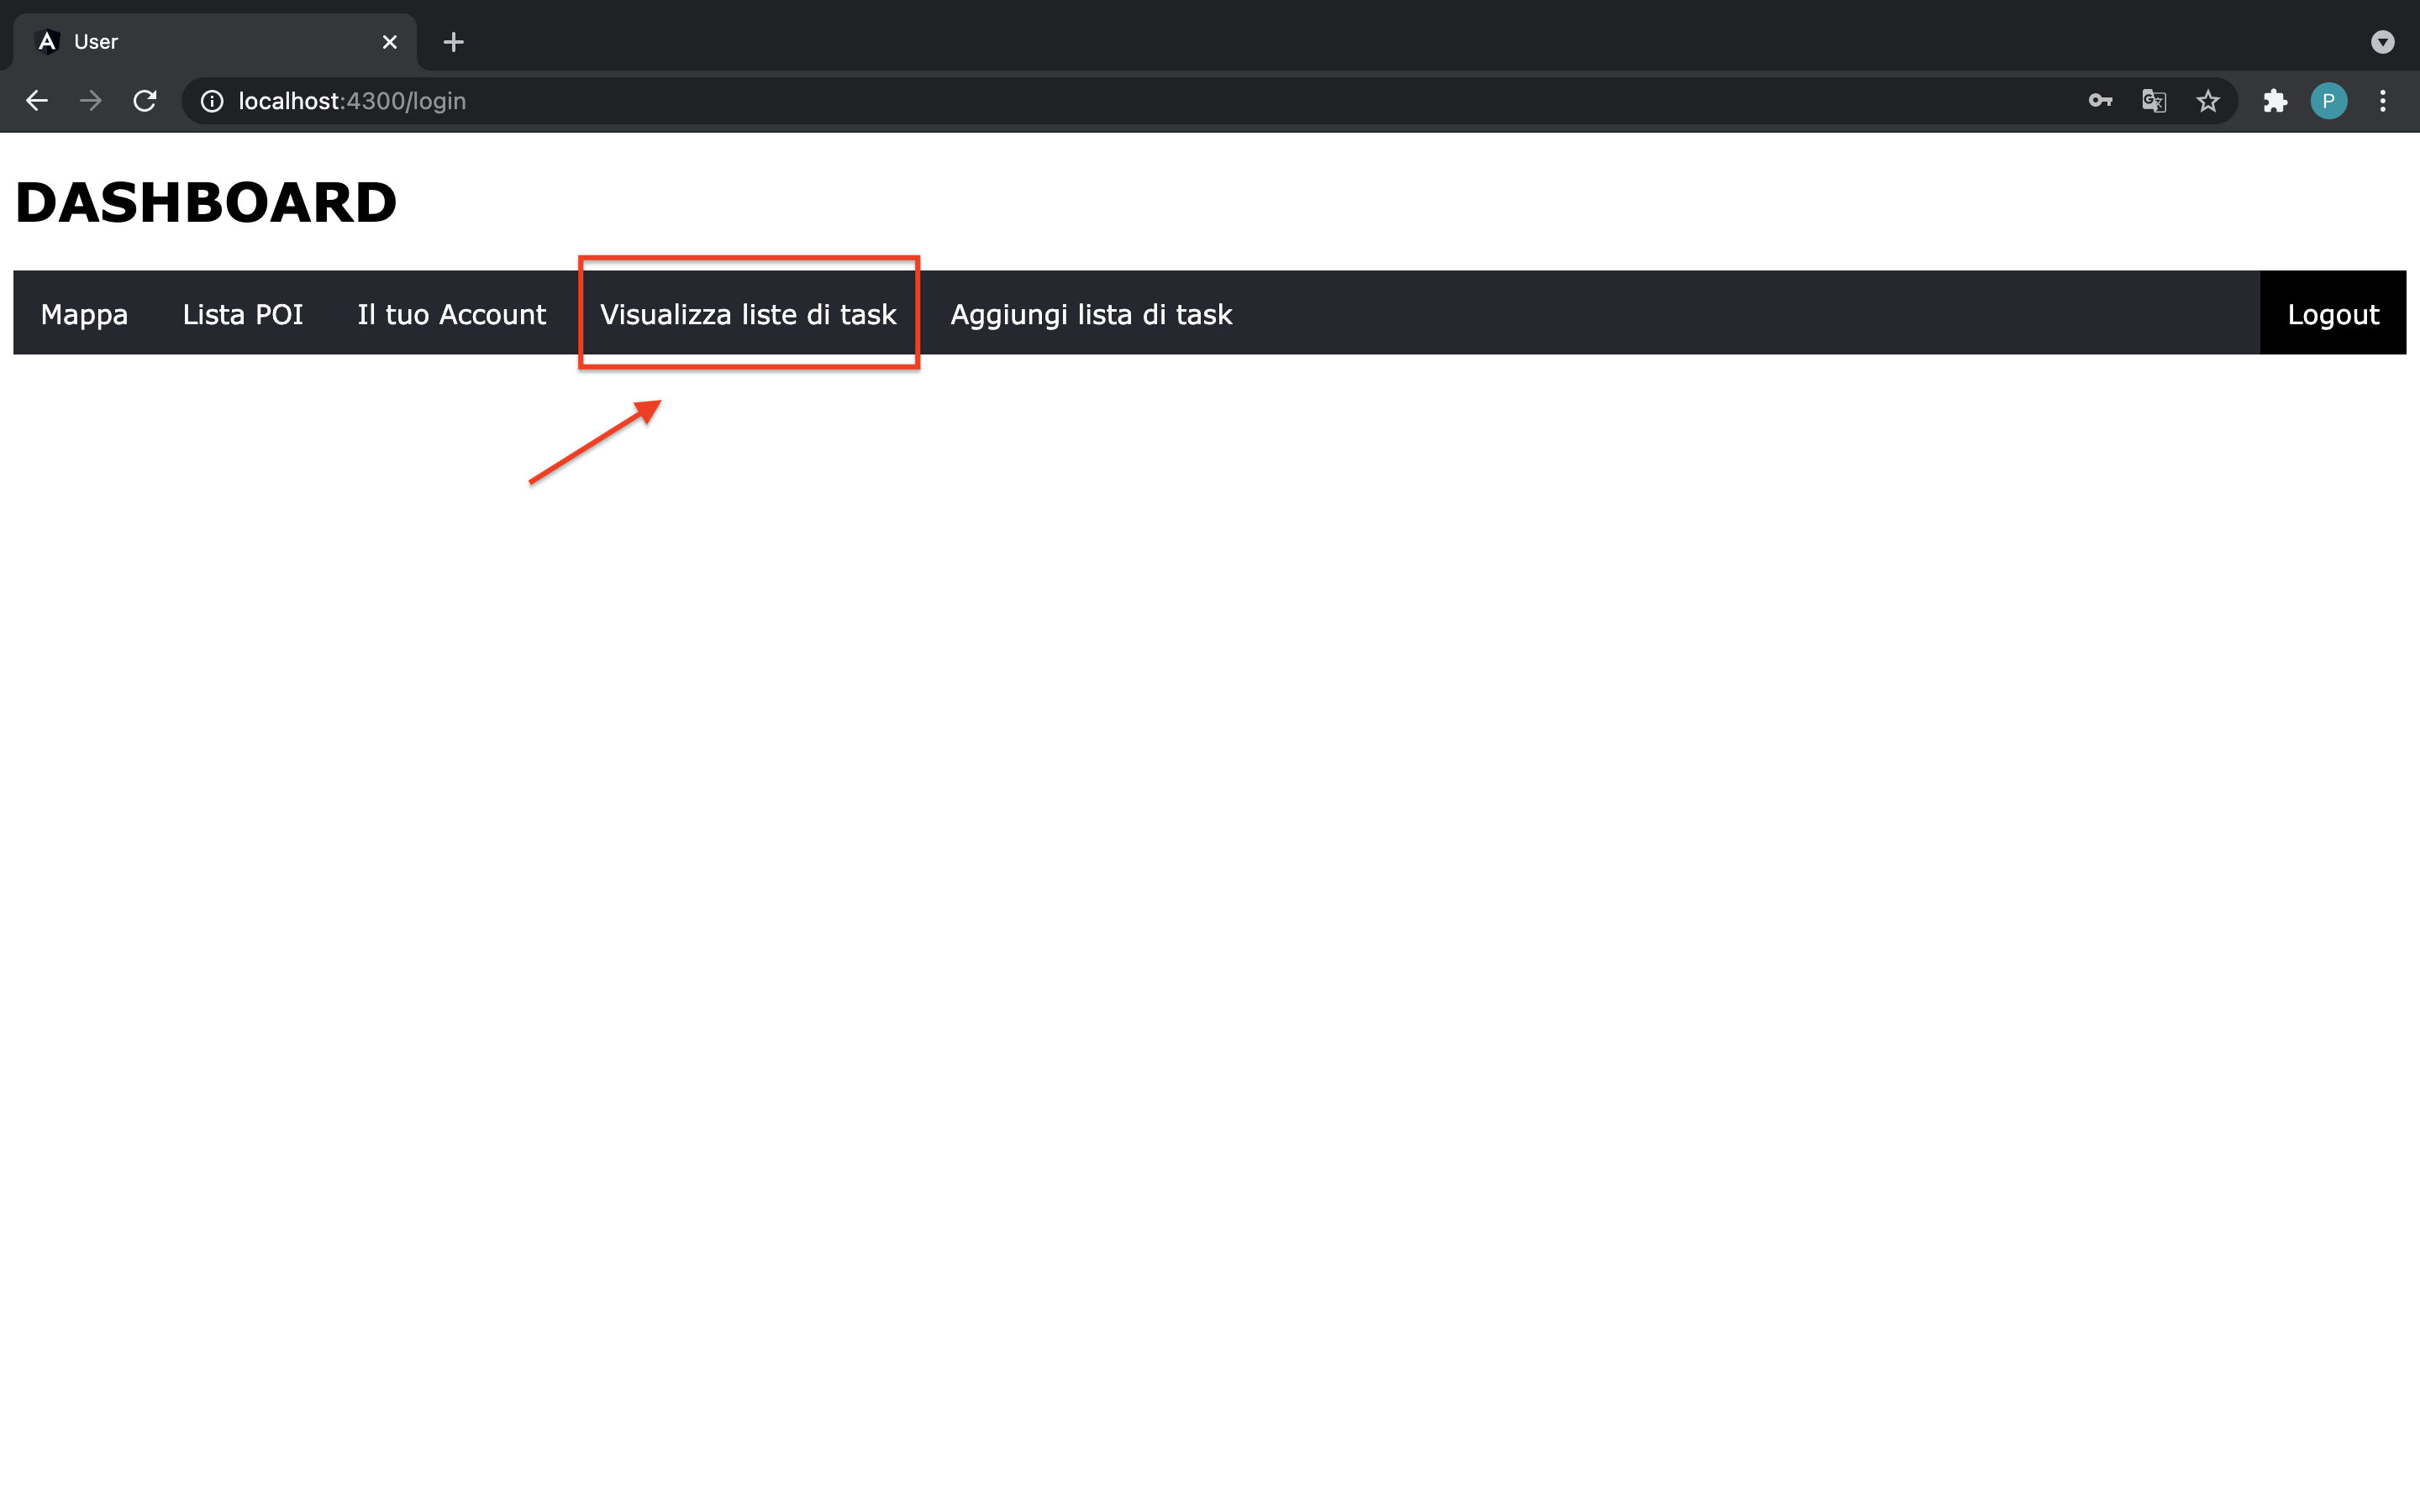
\includegraphics[scale=0.2]{res/images/dashboard8.png}
        \caption{Schermata dashboard con indicazione per la visualizzazione delle task}
    \end{figure}
    \item si viene indirizzati alla pagina con due liste: a sinistra le liste assegnate mentre a destra quelle non assegnate.
    \begin{figure}[H]
        \centering
        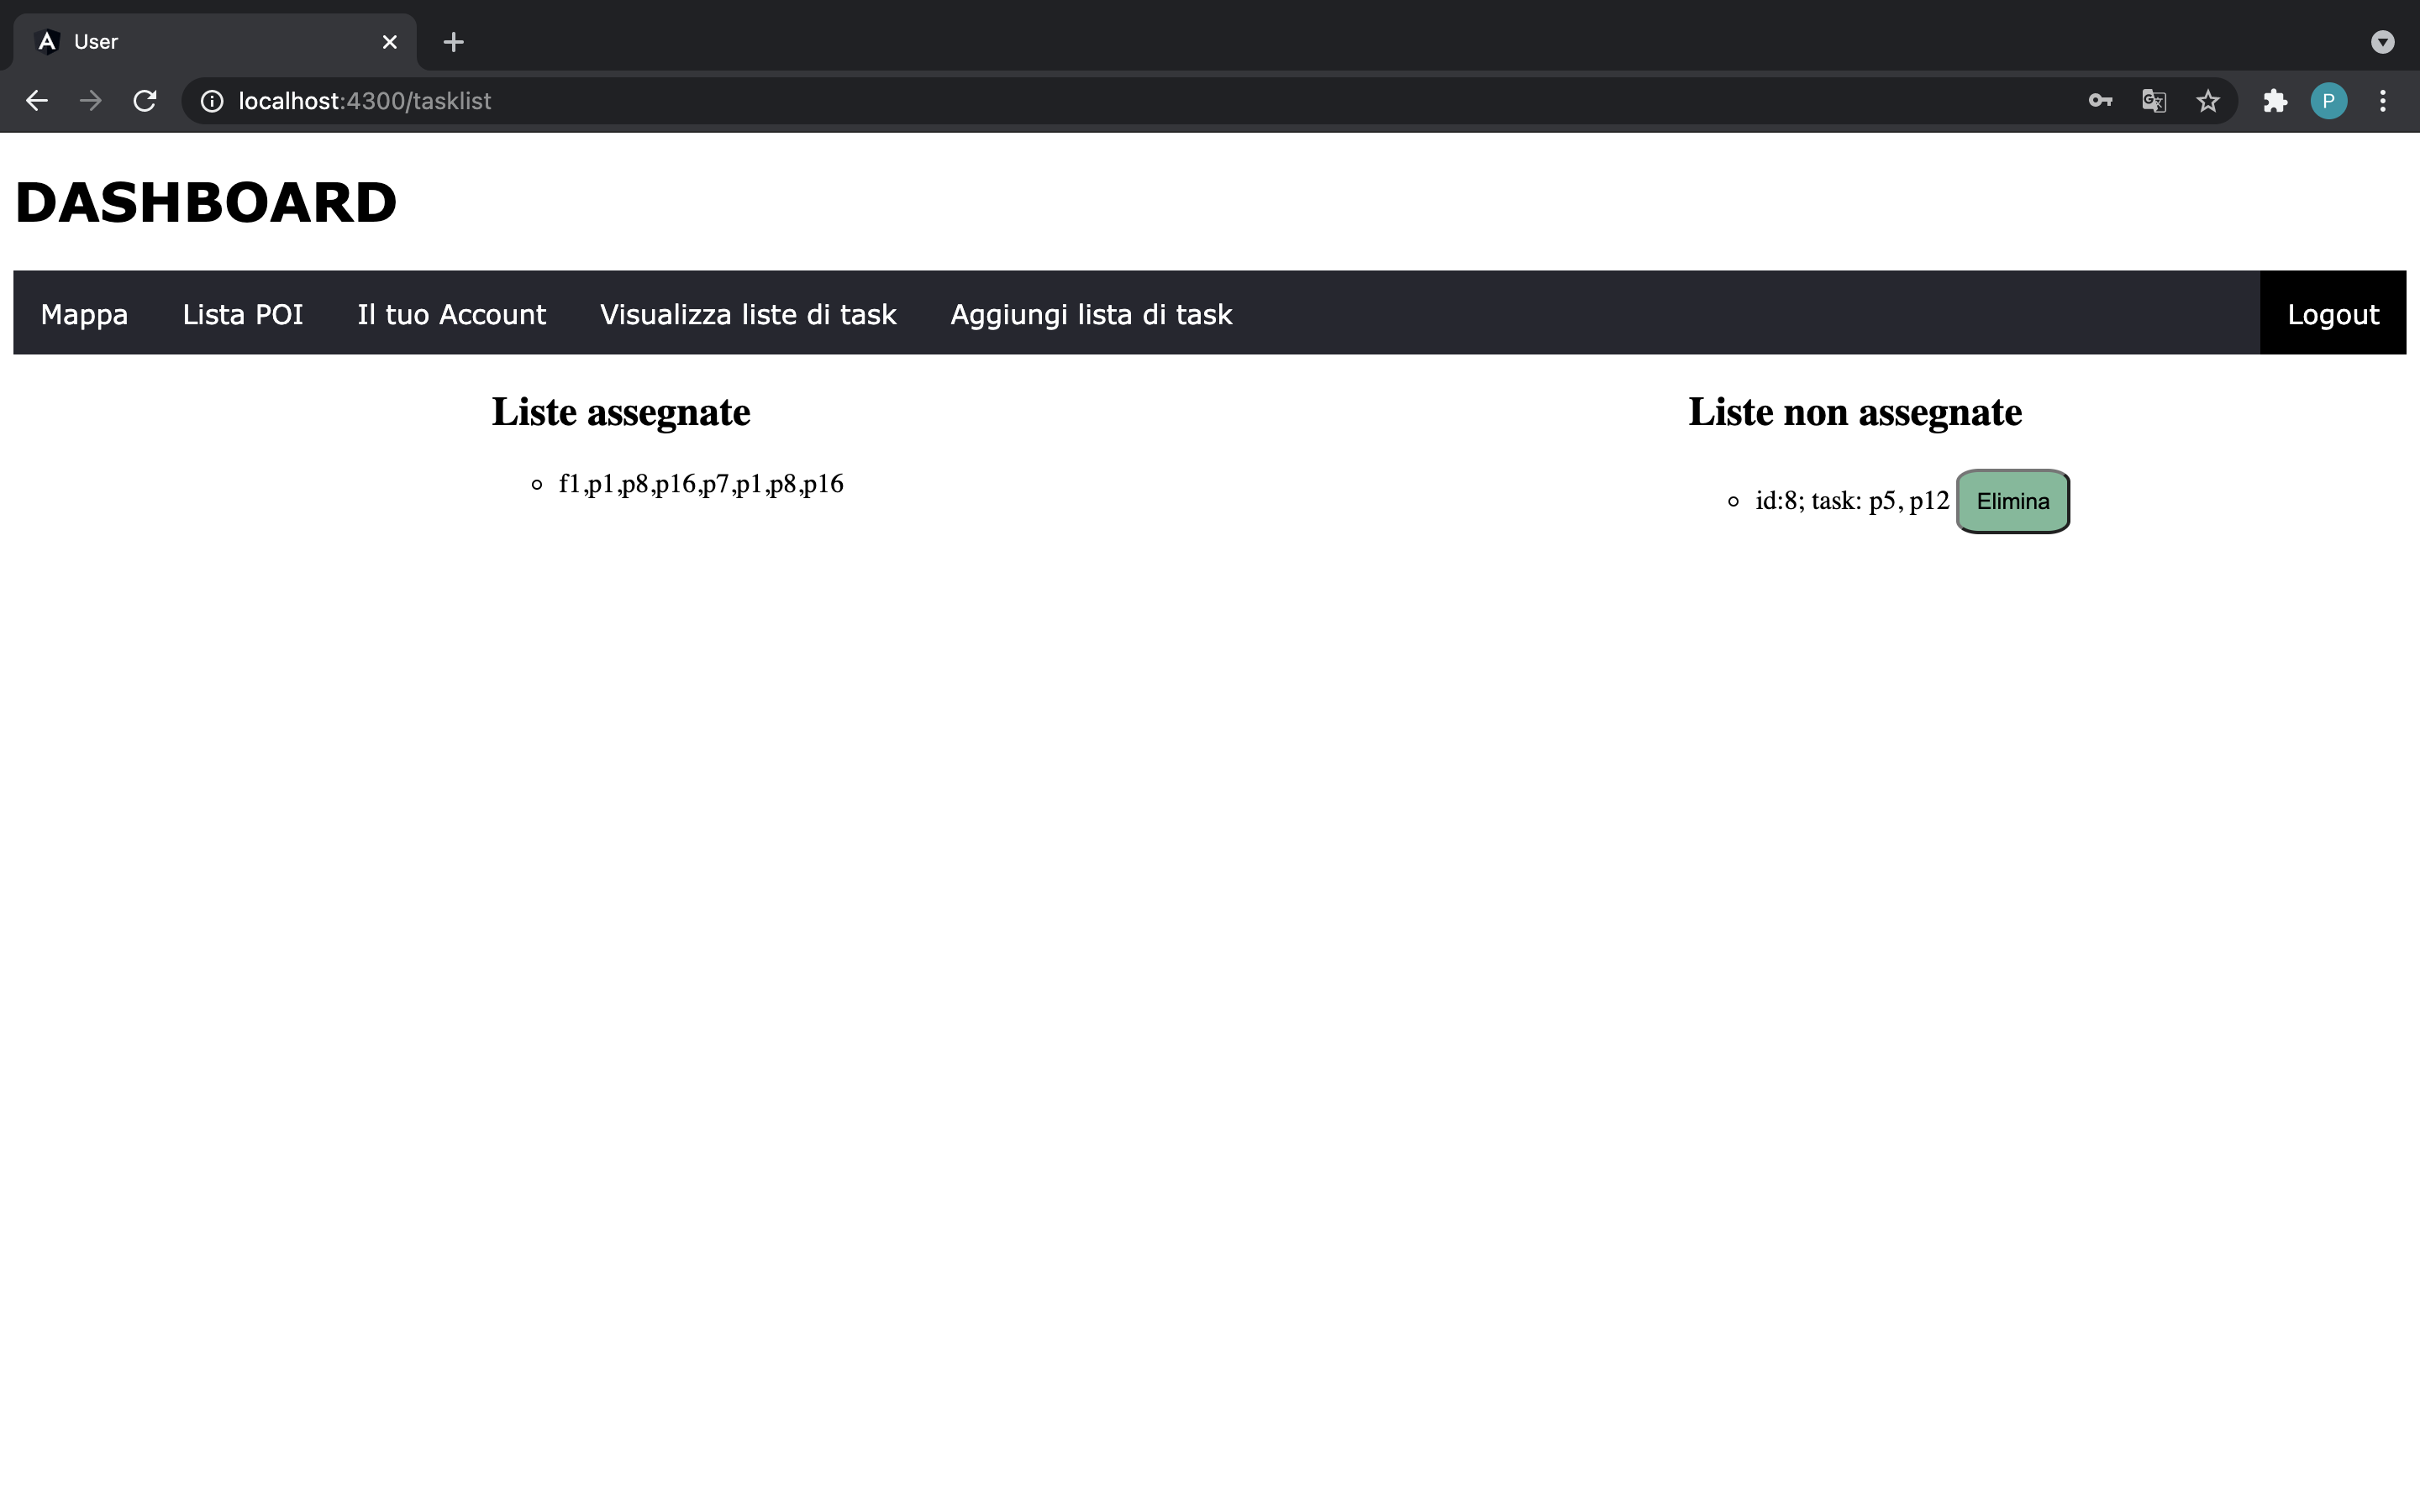
\includegraphics[scale=0.2]{res/images/tasklist.png}
        \caption{Schermata guida automatica dell'unità}
    \end{figure}
    \item è possibile eliminare una lista di task non ancora assegnata a nessun muletto, premendo l'apposito pulsante "Elimina".
    \begin{figure}[H]
        \centering
        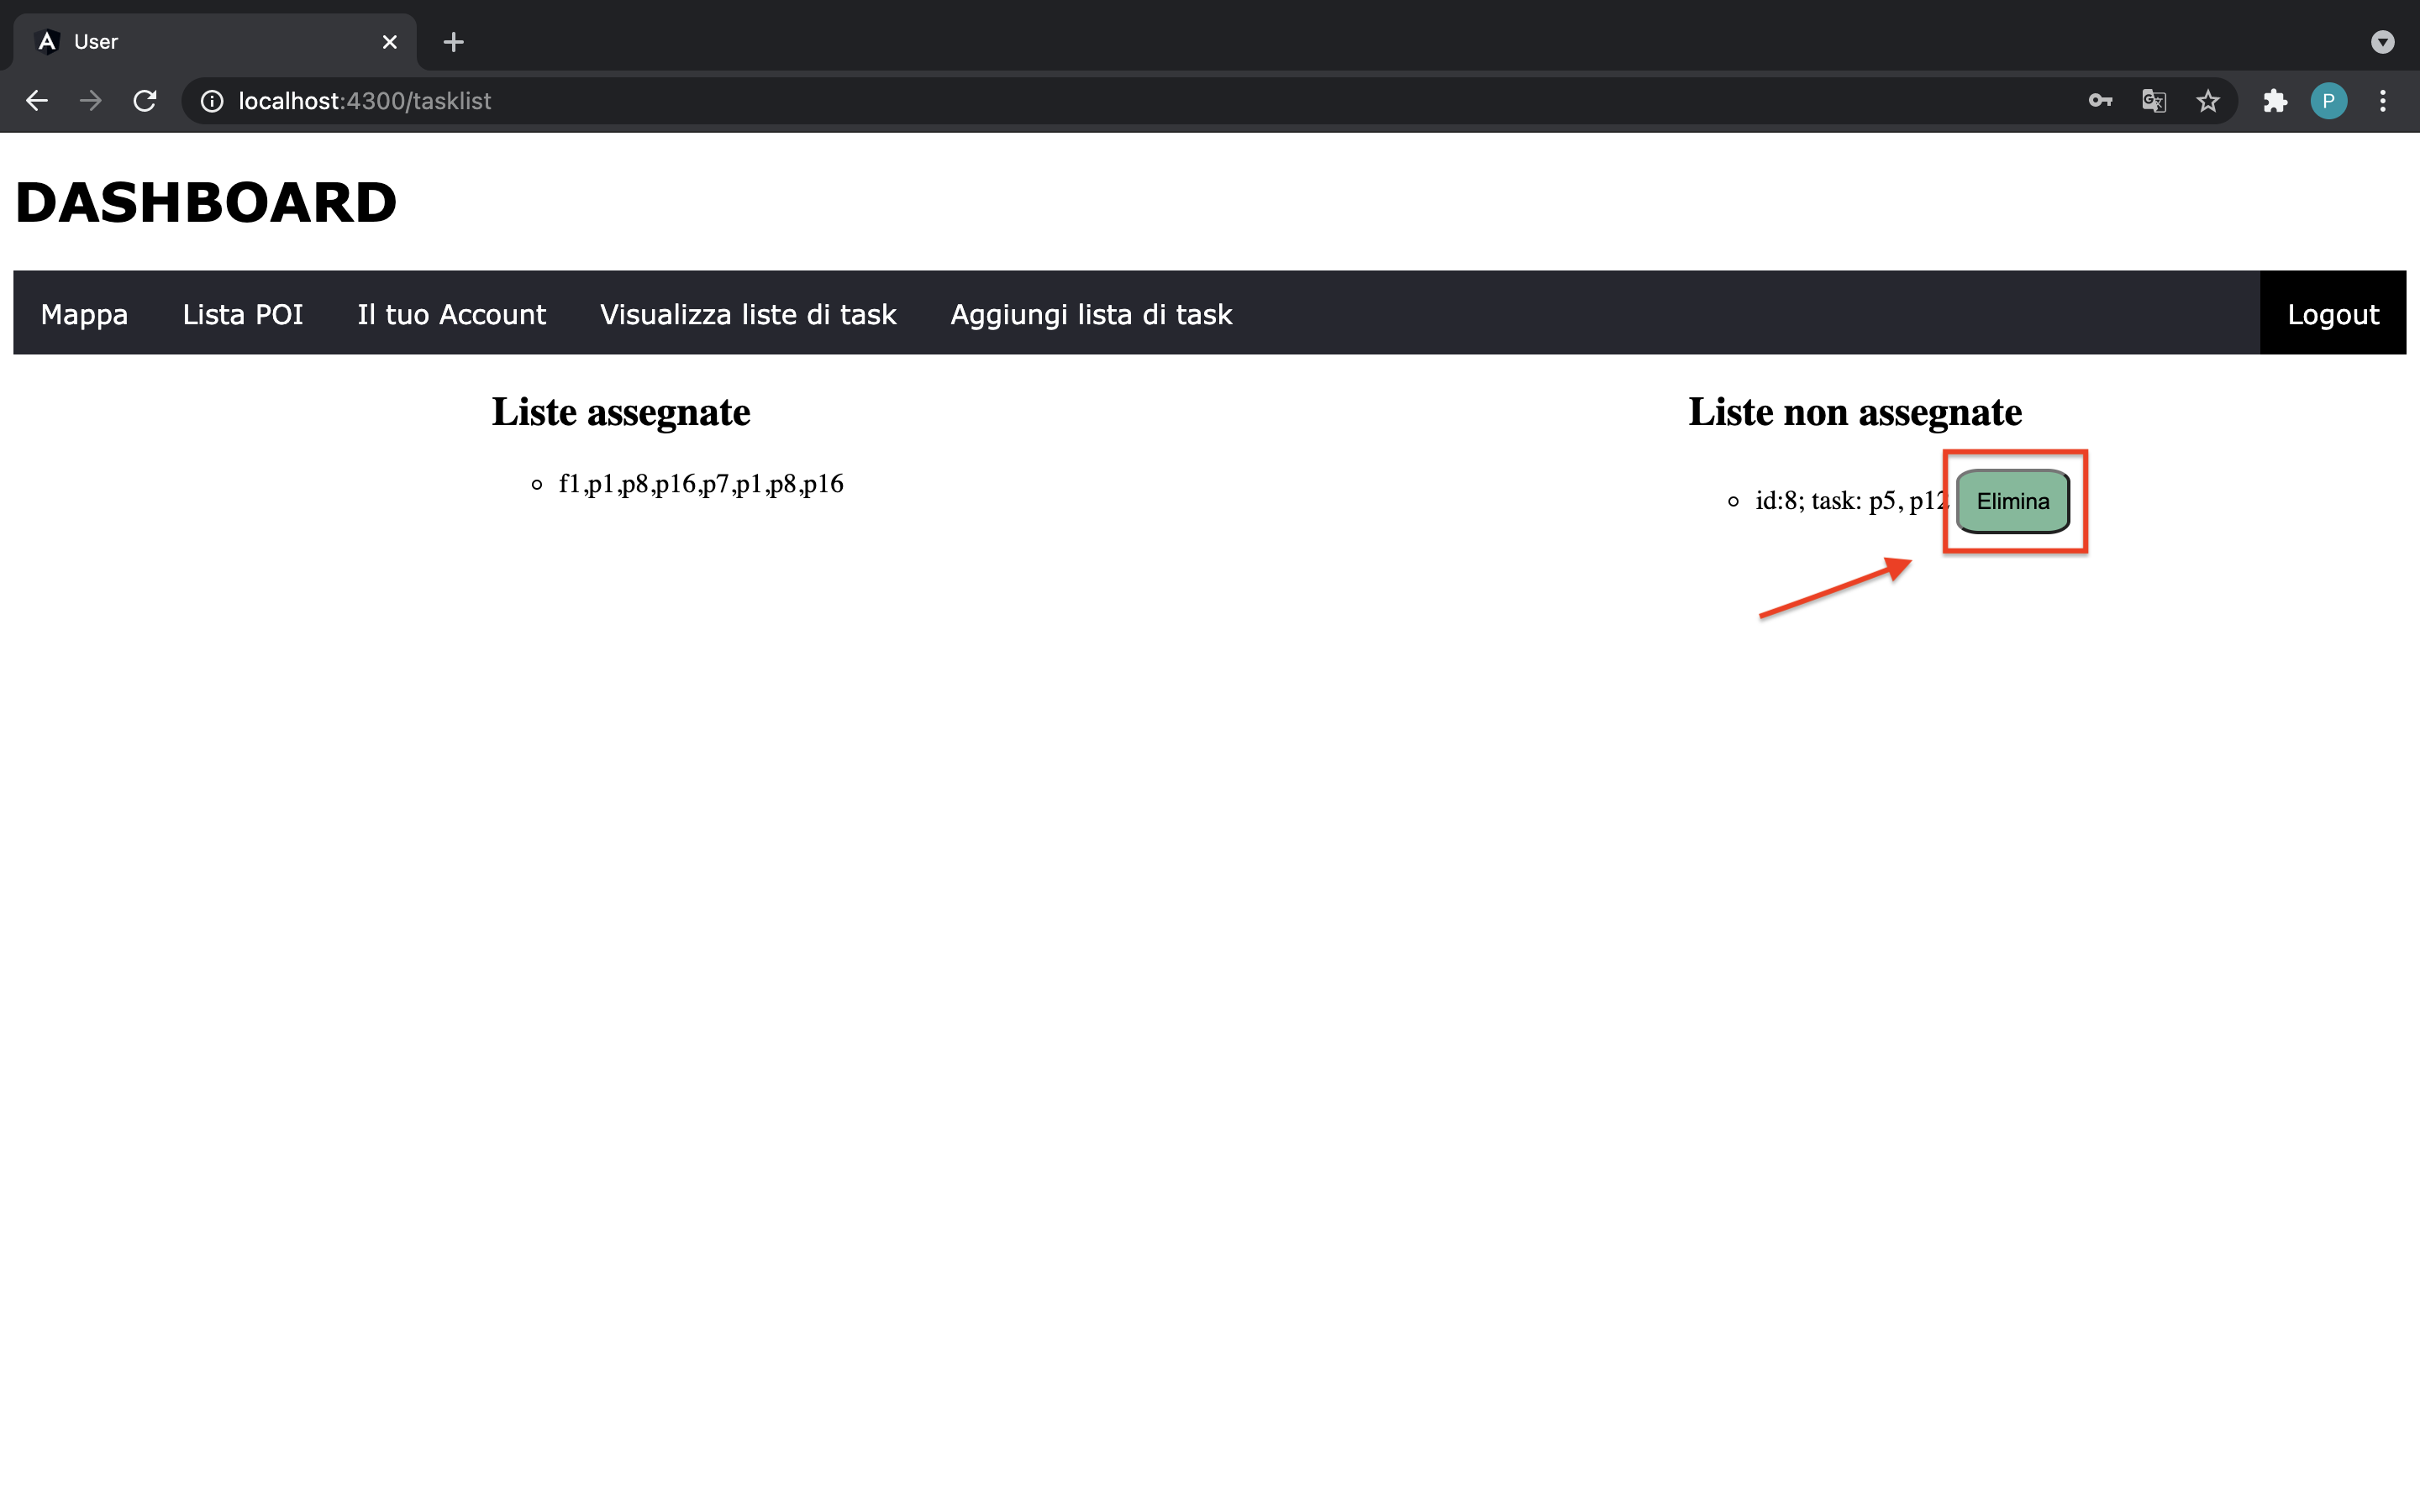
\includegraphics[scale=0.2]{res/images/deletelist.png}
        \caption{Schermata guida automatica dell'unità}
    \end{figure}
    

\subsection{Gestione task}
\begin{itemize}
    \item Dopo l'autenticazione, tramite il menù selezionare il pulsante "Gestisci task";
    \begin{figure}[H]
        \centering
        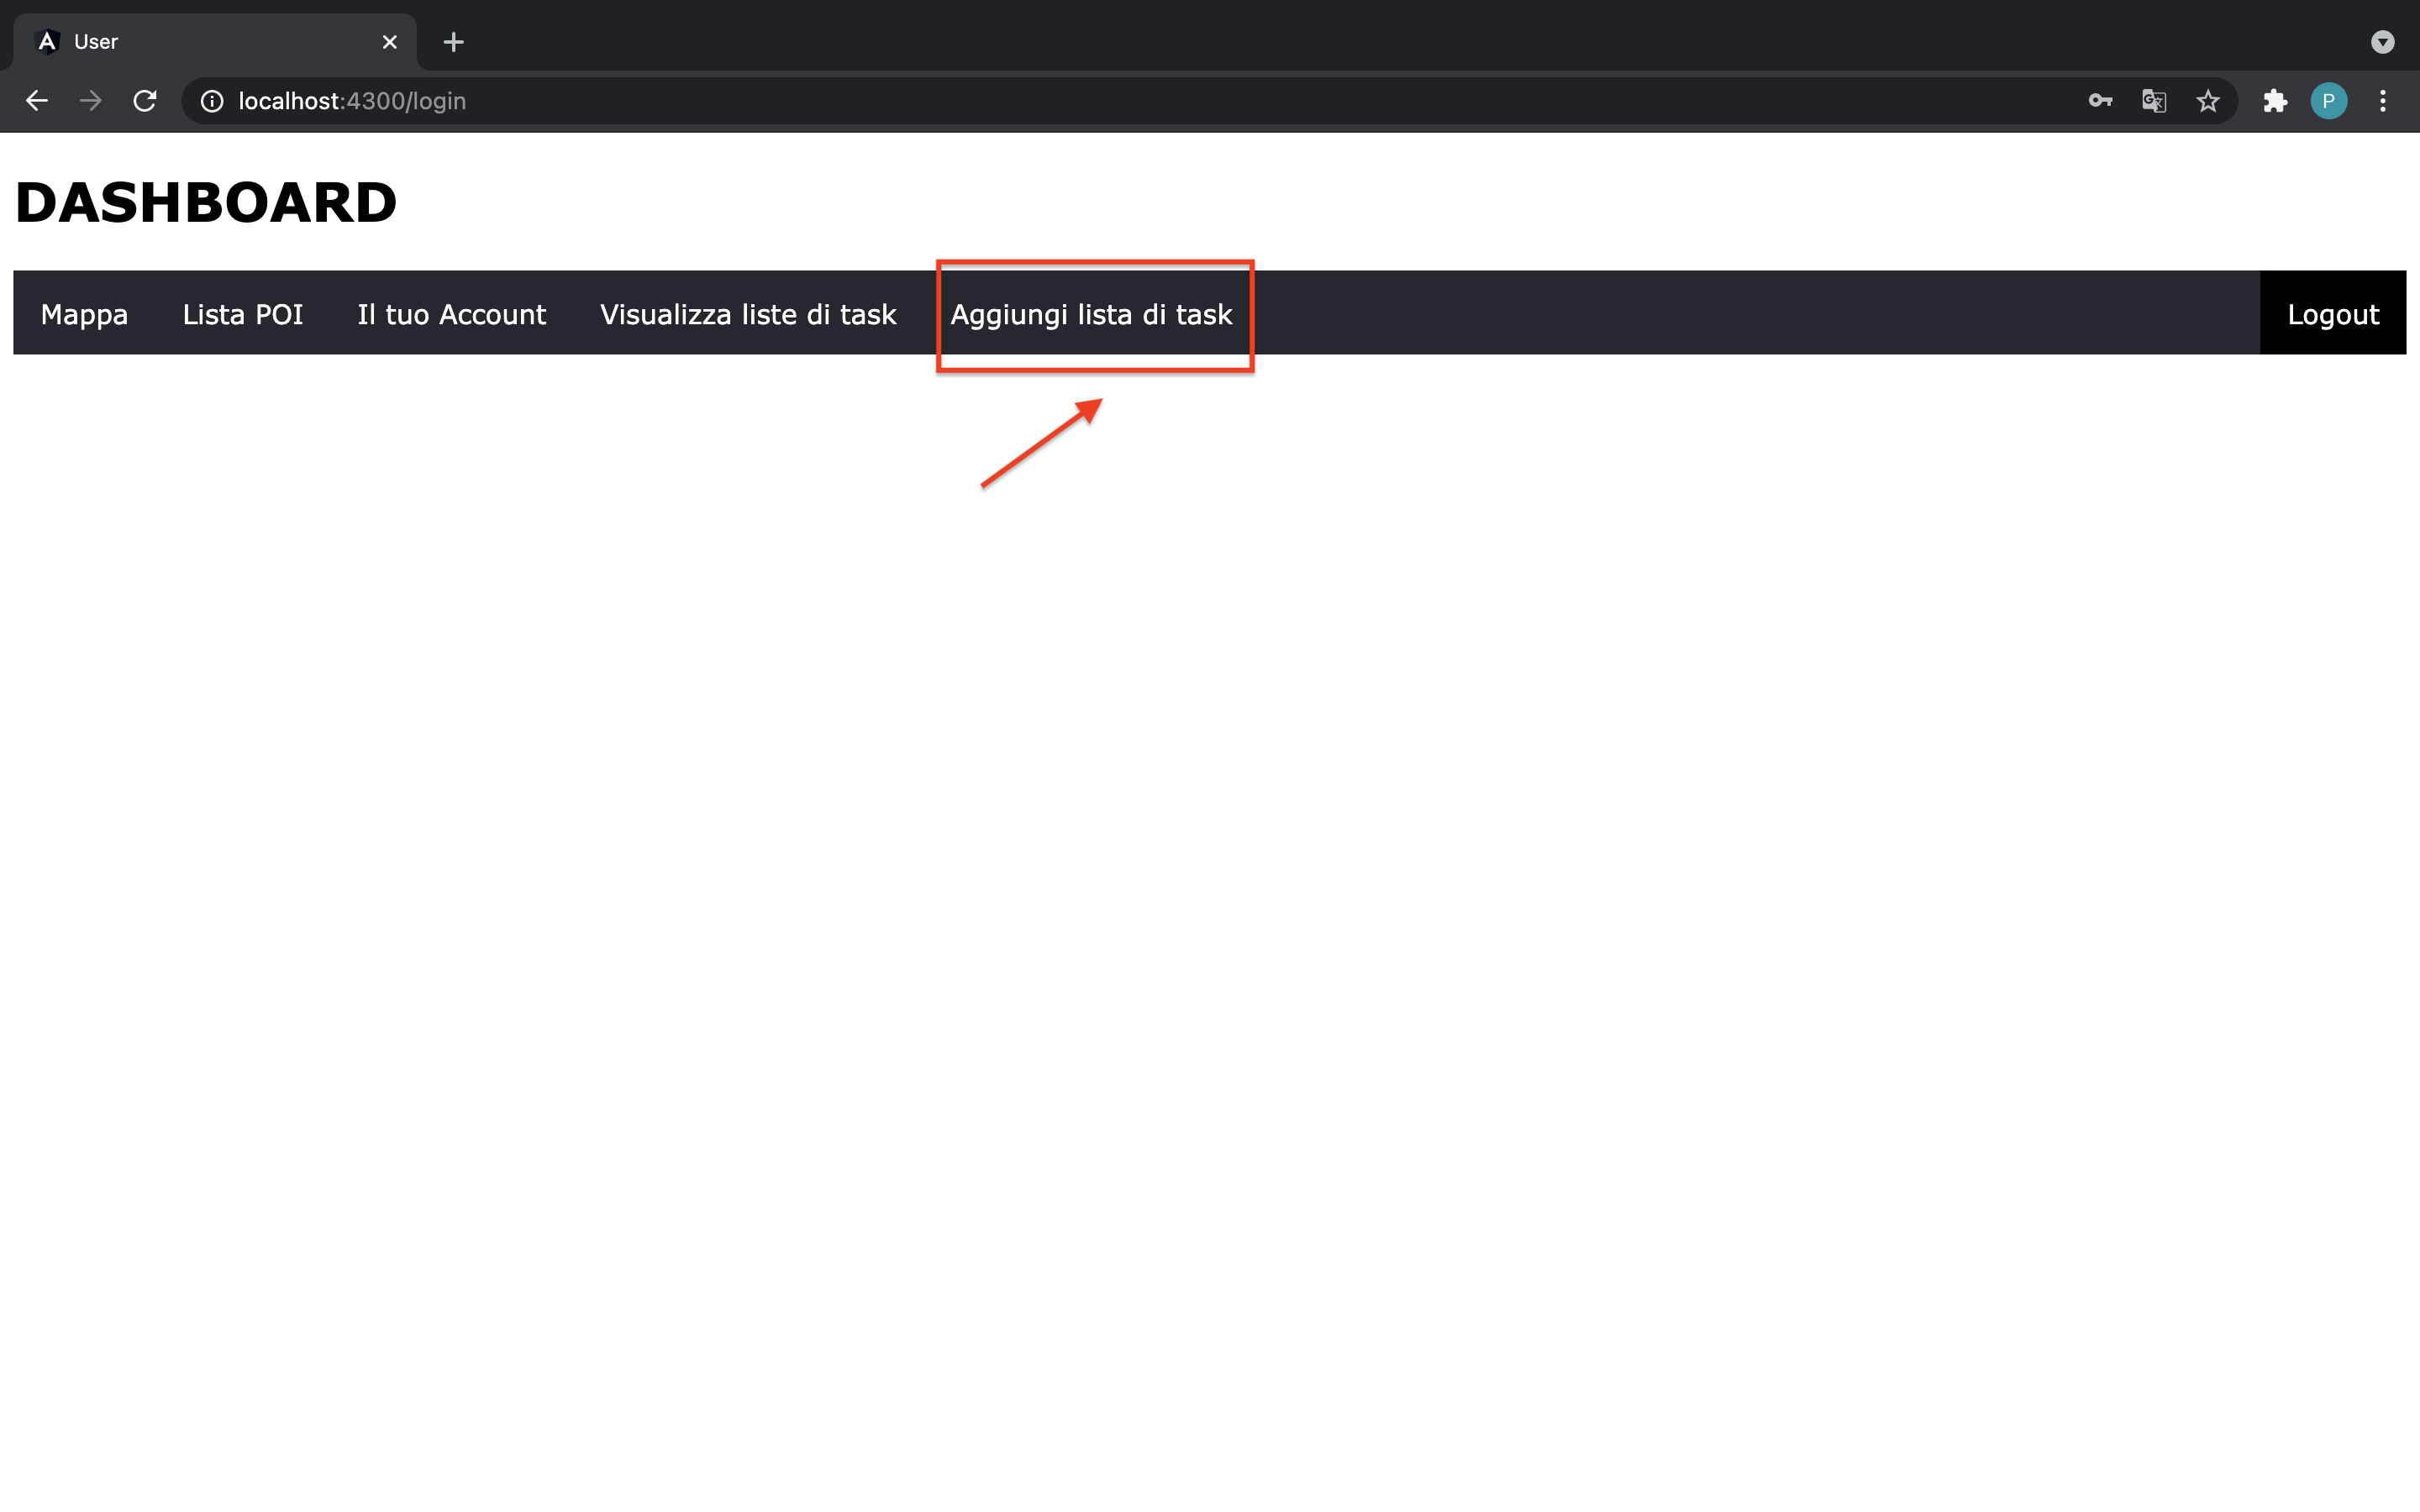
\includegraphics[scale=0.2]{res/images/dashboard9.png}
        \caption{Schermata guida automatica dell'unità}
    \end{figure}
    \item si viene indirizzati alla pagina con le operazioni per la gestione delle task;
    \begin{figure}[H]
        \centering
        \includegraphics[scale=0.2]{res/images/gestiscitask.png
        \caption{Schermata per la gestione delle task}
    \end{figure}
\end{itemize}
\subsubsection{Aggiungere nuova lista di task}
\begin{itemize}
   
    \item viene visualizzato un menu a tendina per selezionare  il POI di interesse e confermare; \\ripetere questo punto per tutte le task che si intendono inserire;
    \begin{figure}[H]
        \centering
        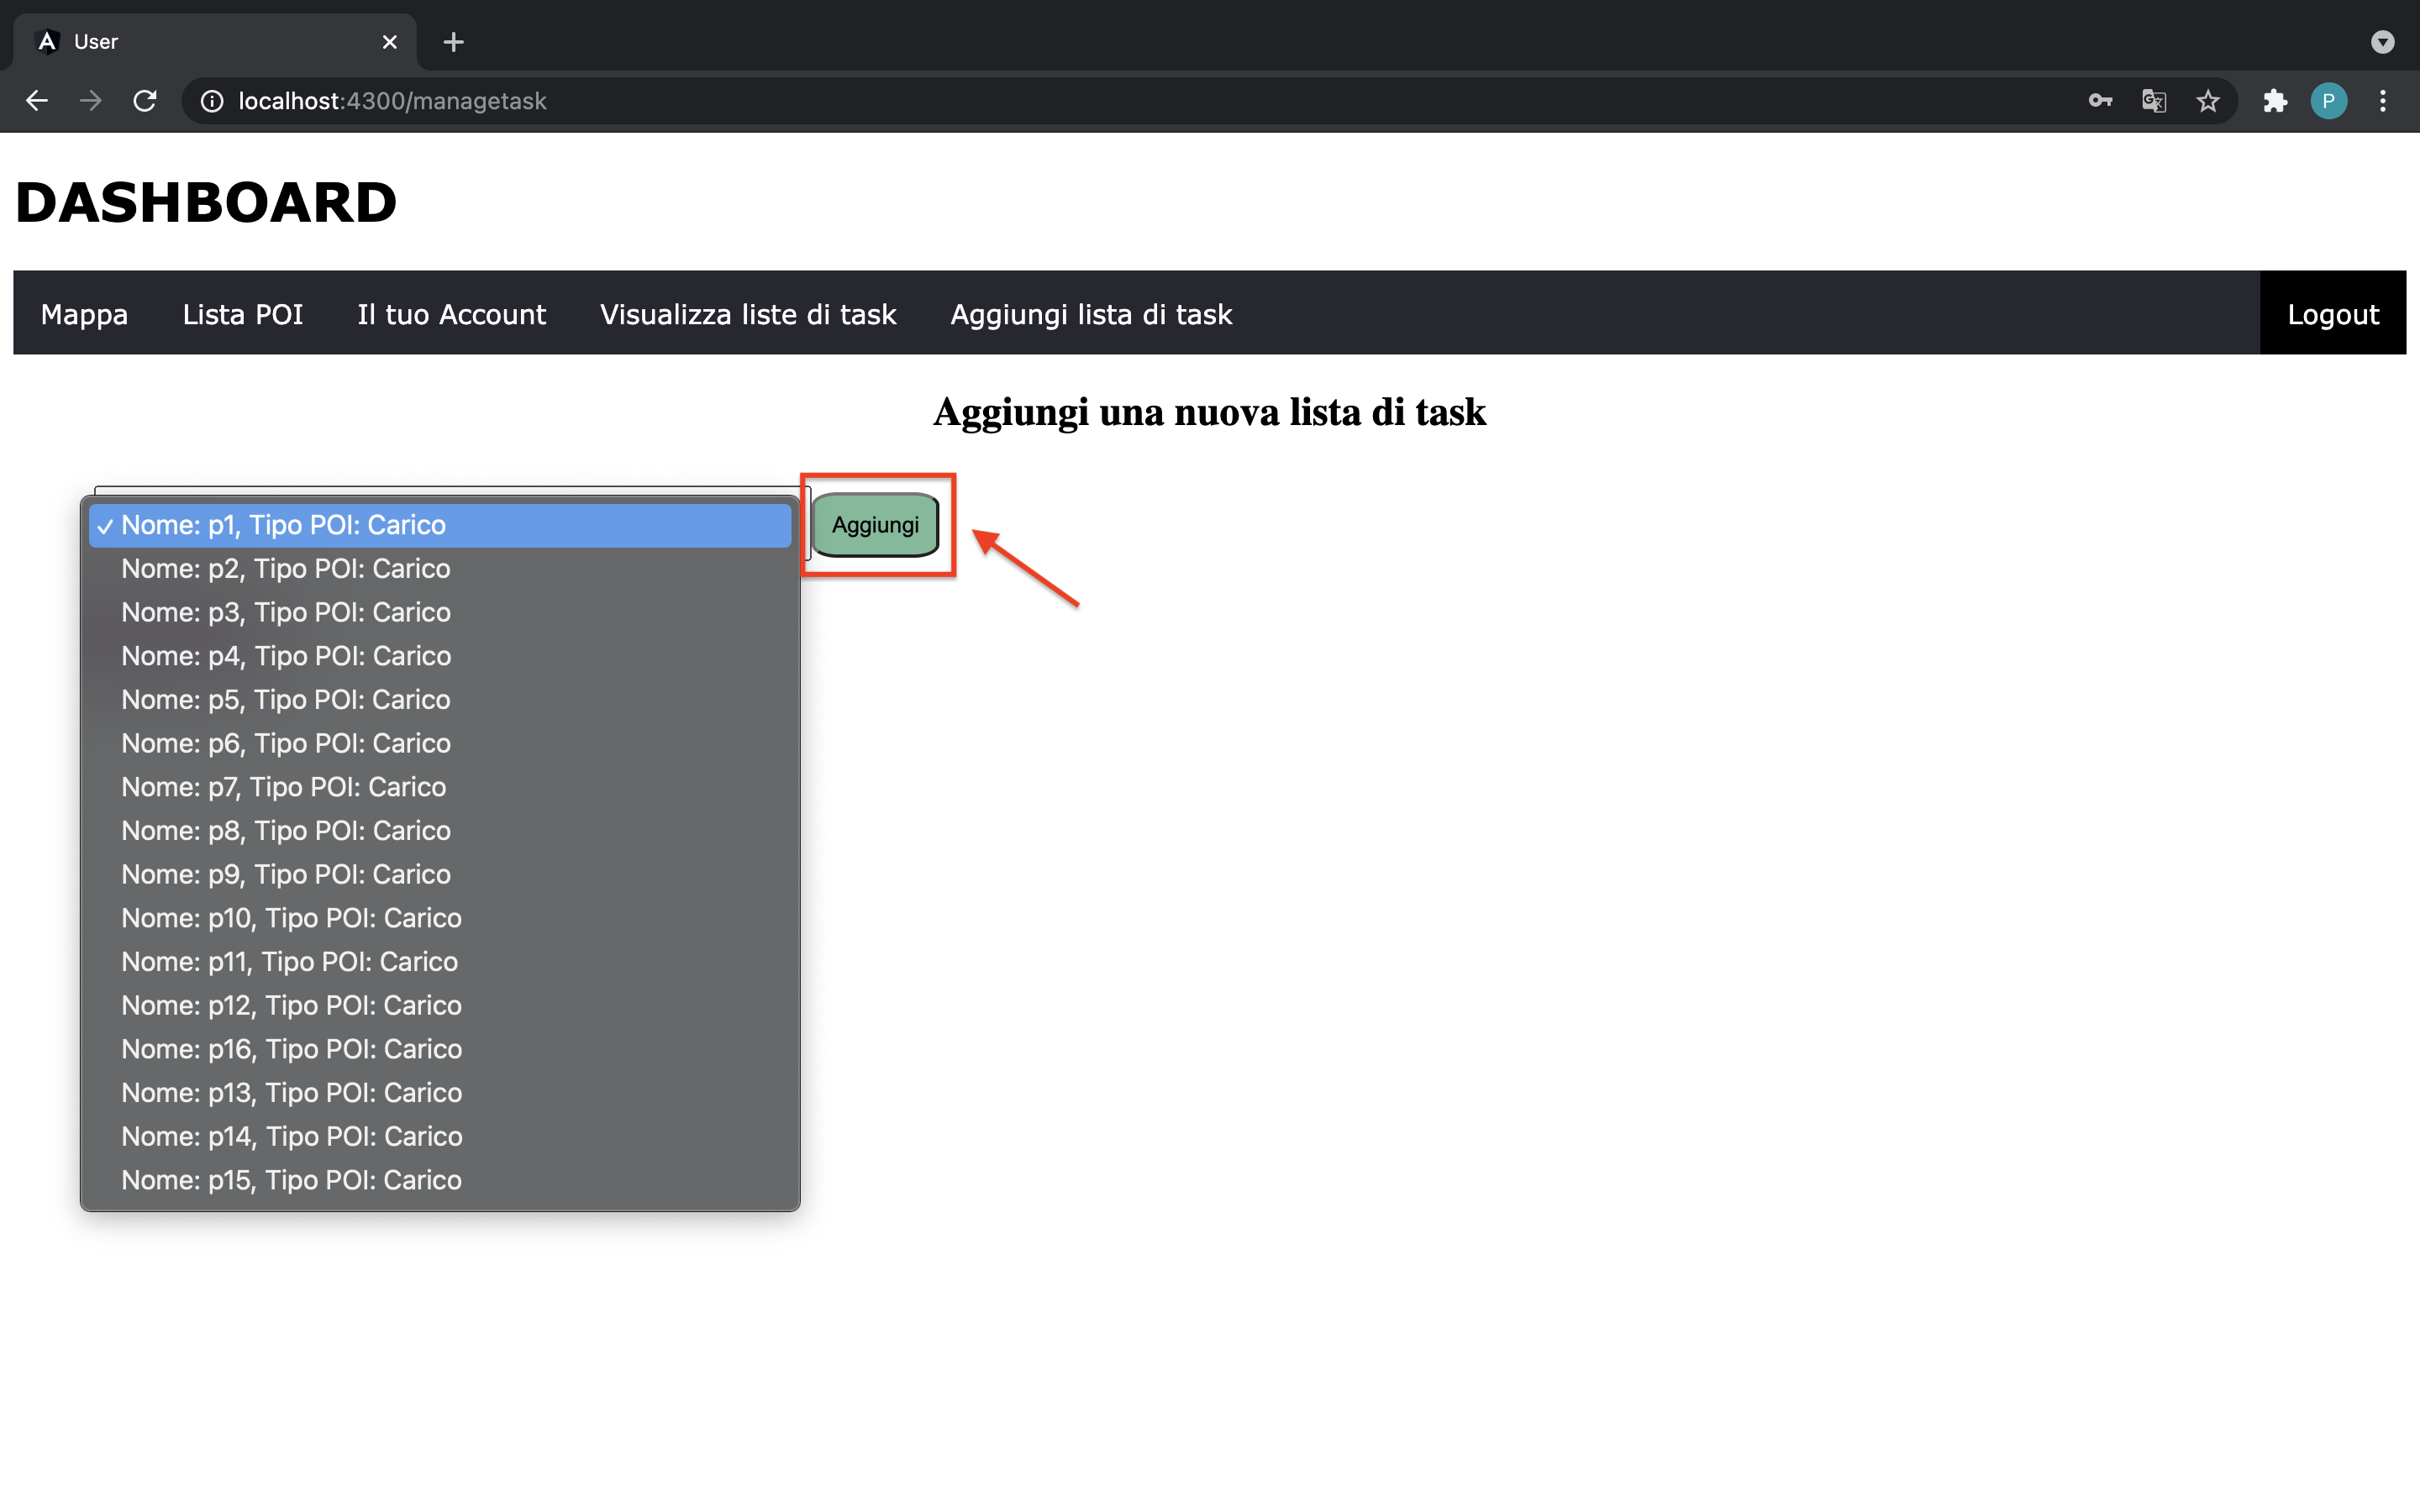
\includegraphics[scale=0.2]{res/images/aggiungitask.png}
        \caption{Schermata per l'aggiunta di una task alla lista che si intende creare}
    \end{figure}
    \item tramite il pulsante "Elimina" di fianco ad ogni task inserita è possibile eliminarla prima di confermare;
    \begin{figure}[H]
        \centering
        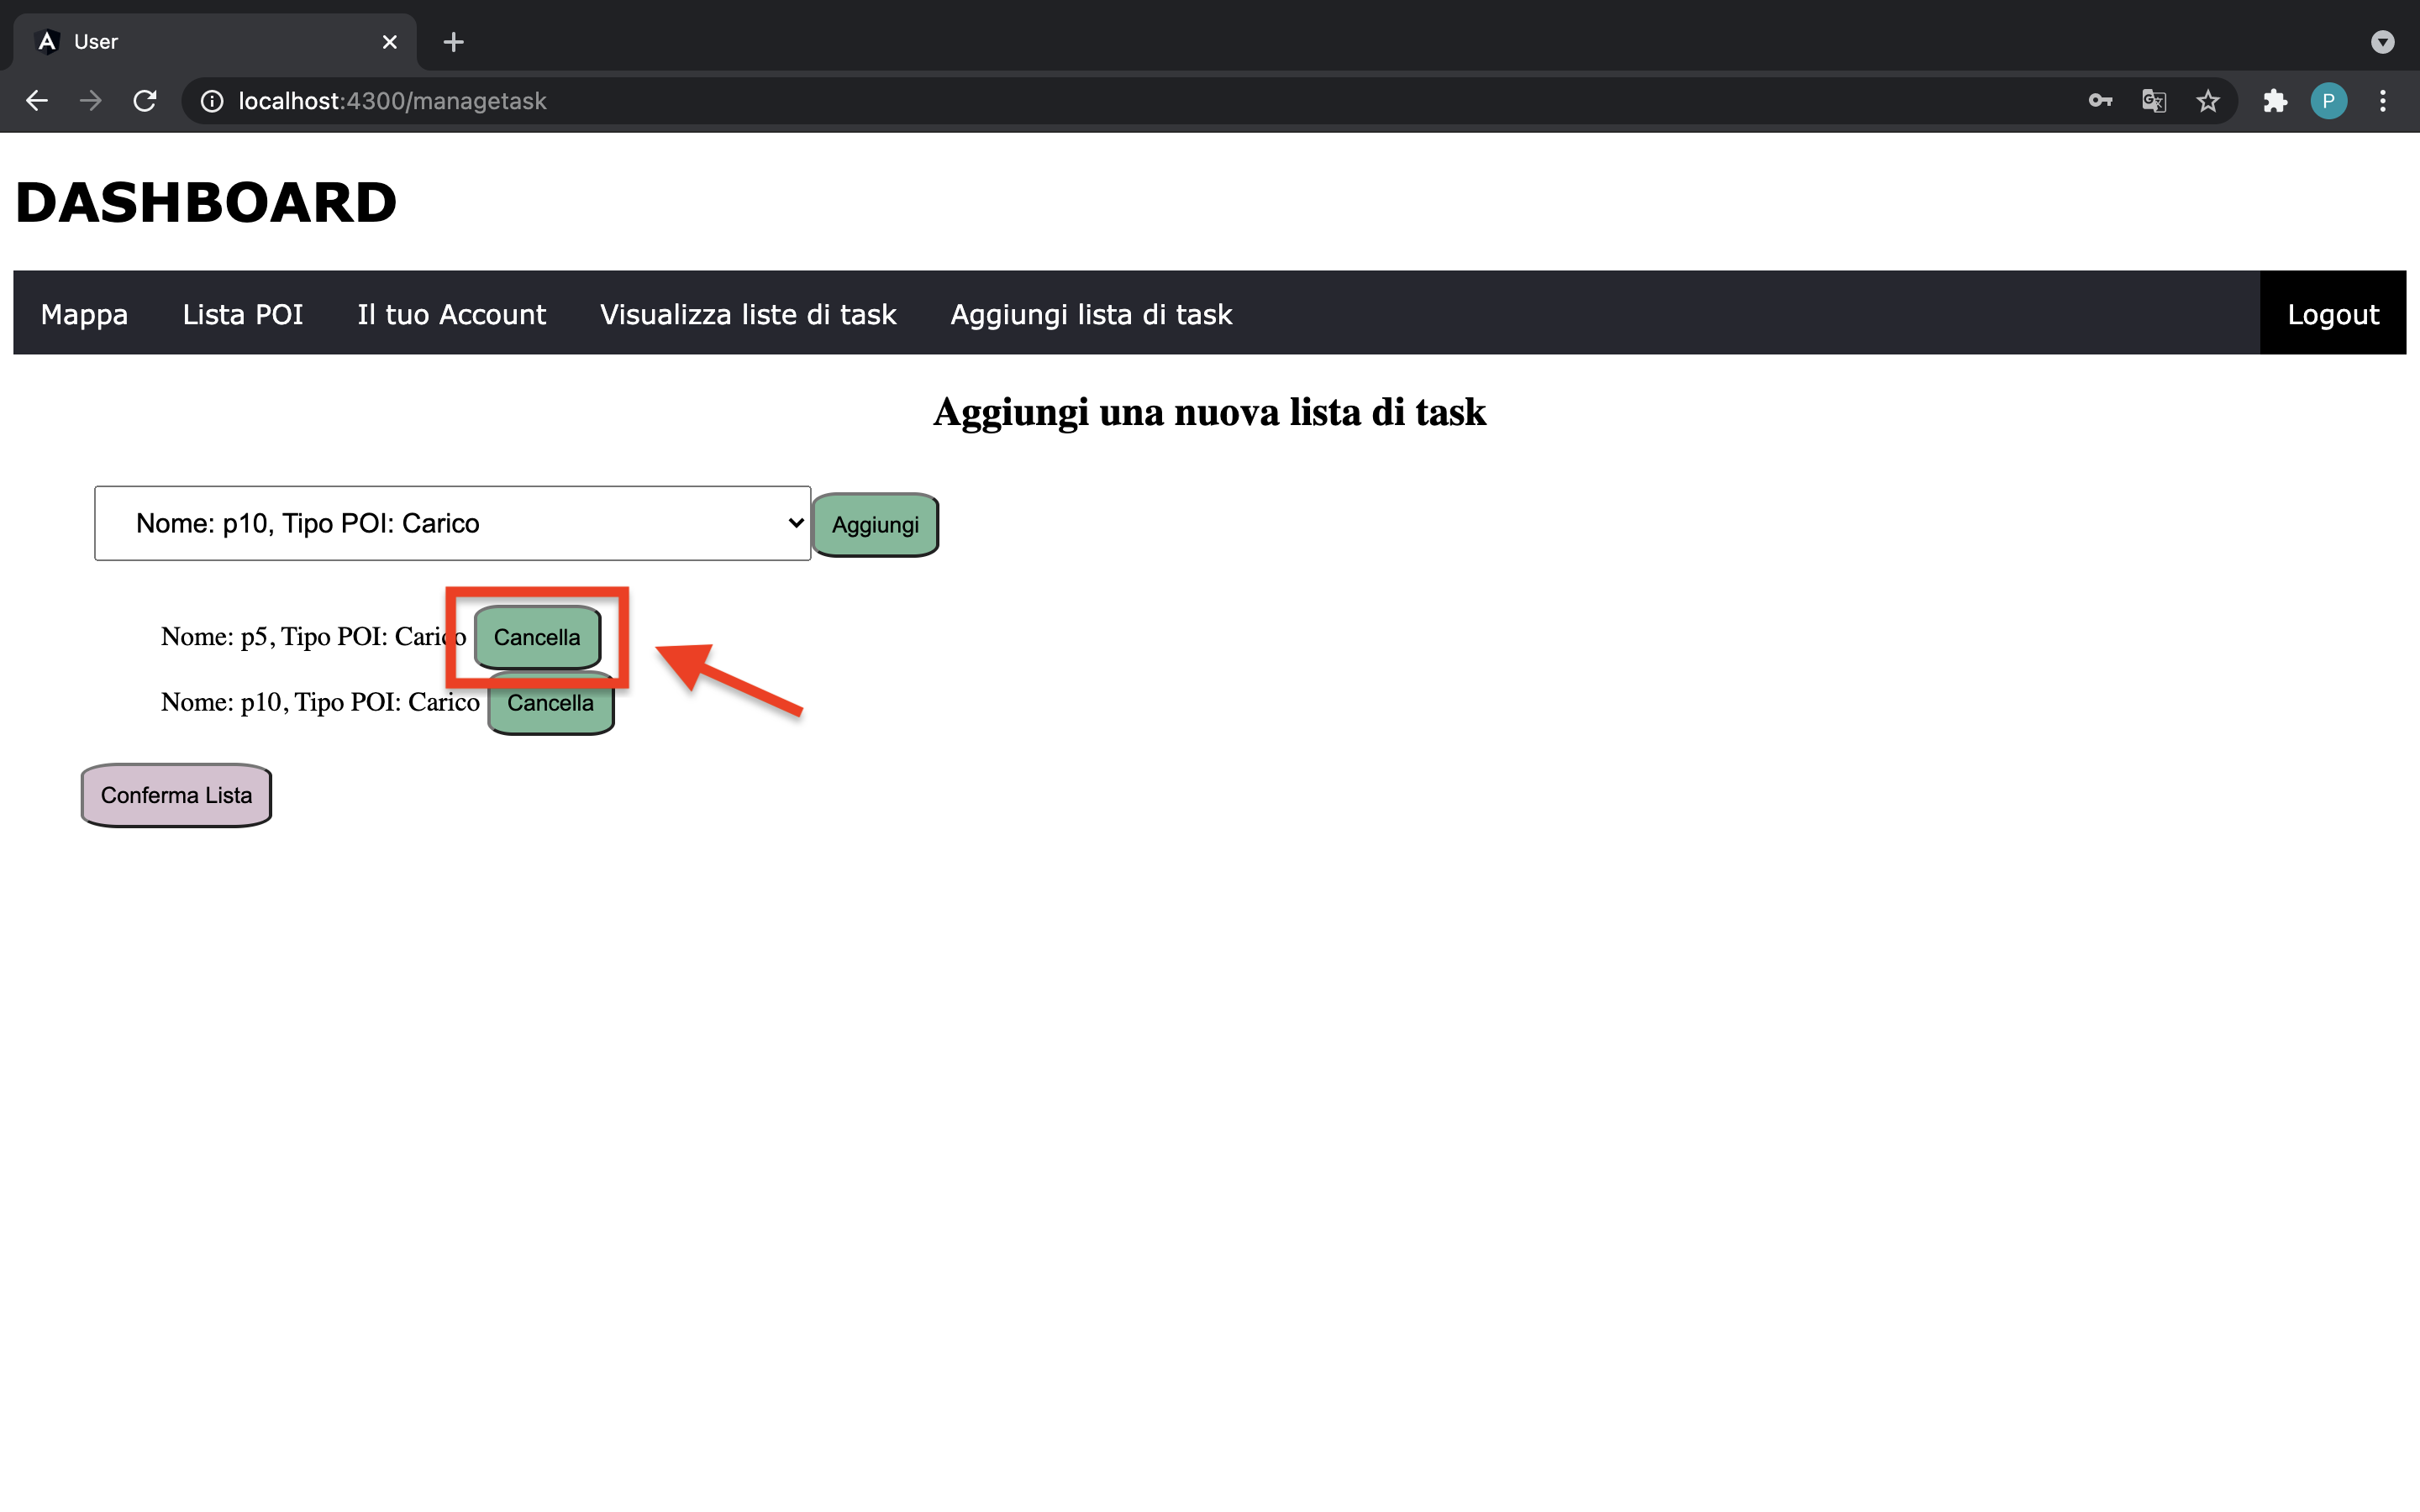
\includegraphics[scale=0.2]{res/images/eliminatask.png}
        \caption{Schermata per l'eliminazione di una task dalla lista che si sta creando}
    \end{figure}
    \item una volta aggiunte tutte le task, premere il pulsante "Conferma";
    \begin{figure}[H]
        \centering
        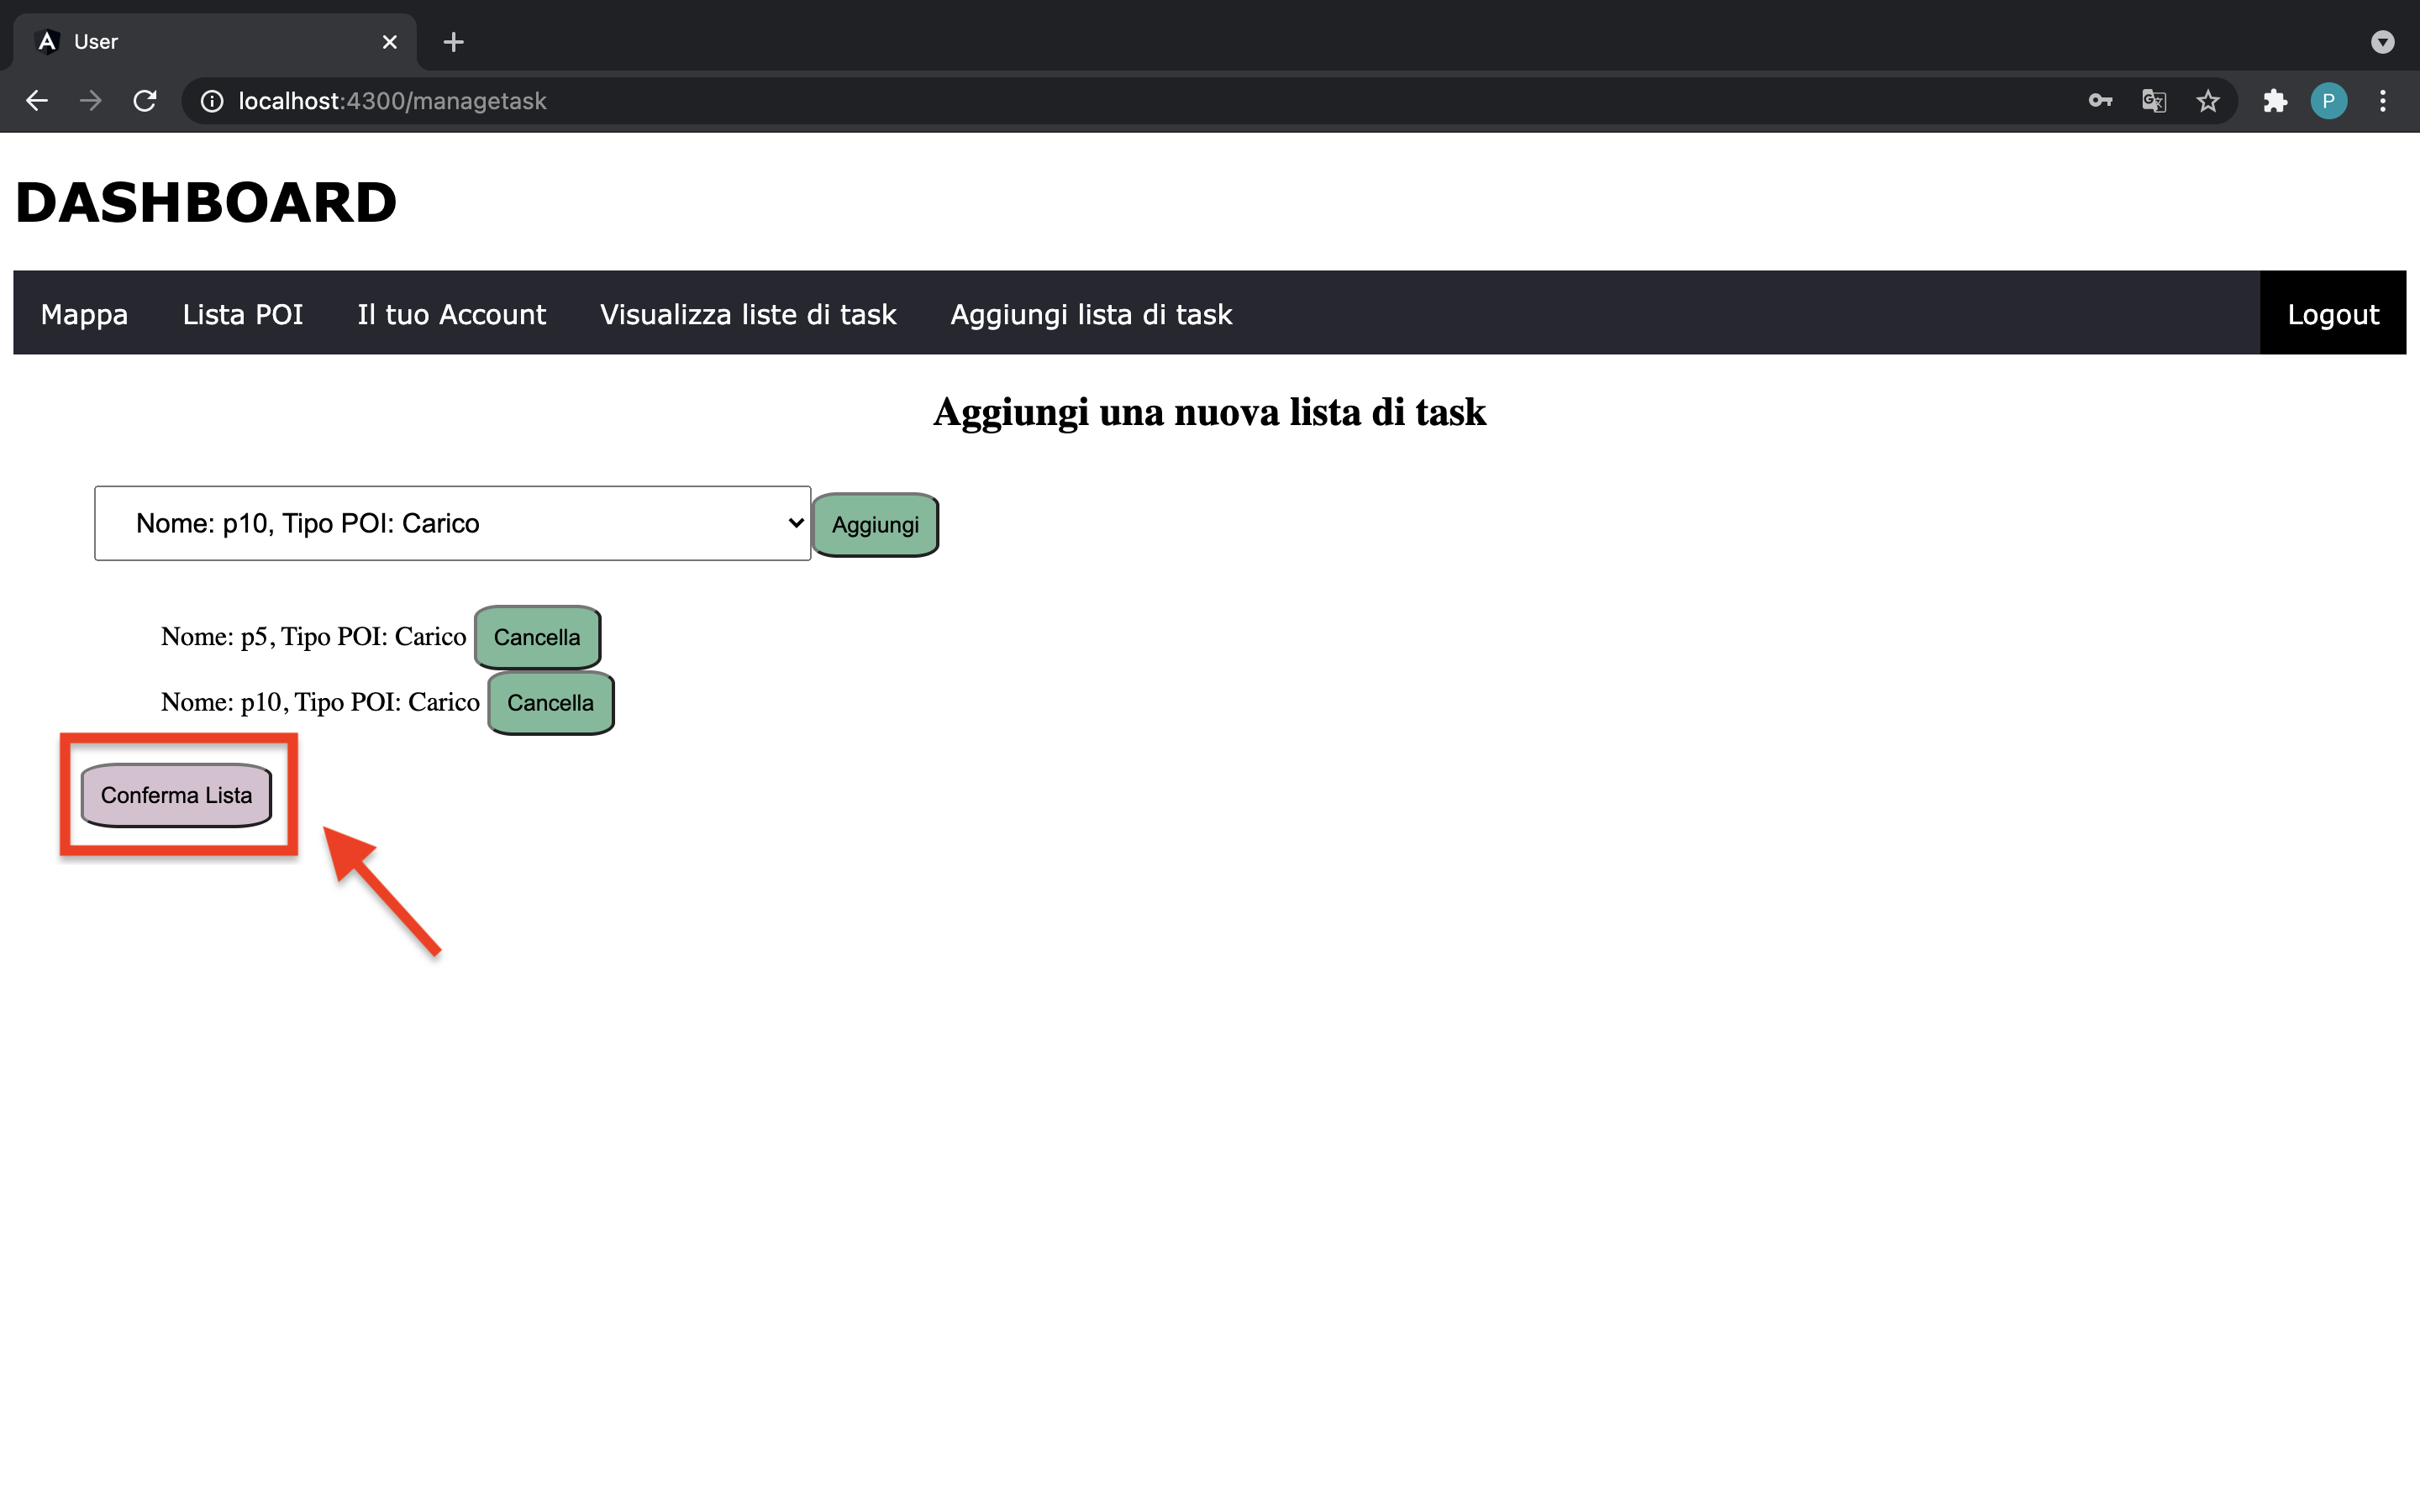
\includegraphics[scale=0.2]{res/images/confermalista.png}
        \caption{Schermata per la conferma della lista di task che si sta creando}
    \end{figure}
    \item una volta ricevuta la lista, si visualizza l'id di essa.
    \begin{figure}[H]
        \centering
        \includegraphics[scale=0.2]{res/images/listacreata.png
        \caption{Schermata conferma creazione lista}
    \end{figure}
\end{itemize}



